\documentclass[oneside,numbers,spanish]{ezthesis}

\usepackage{lmodern,textcomp}
\usepackage[T1]{fontenc}
\usepackage[spanish,activeacute]{babel}
\usepackage{mathtools}
\usepackage[utf8x]{inputenc}
\usepackage{enumerate}
\usepackage{float}
\usepackage[normalem]{ulem}
\usepackage{eurosym}
\usepackage{multirow}
\usepackage{url}
\usepackage{lscape}
\usepackage{listings}




\useunder{\uline}{\ul}{}

%% # Opciones disponibles para el documento #
%%
%% Las opciones con un (*) son las opciones predeterminadas.
%%
%% Modo de compilar:
%%   draft            - borrador con marcas de fecha y sin im'agenes
%%   draftmarks       - borrador con marcas de fecha y con im'agenes
%%   final (*)        - version final de la tesis
%%
%% Tama'no de papel:
%%   letterpaper (*)  - tama'no carta (Am'erica)
%%   a4paper          - tama'no A4    (Europa)
%%
%% Formato de impresi'on:
%%   oneside          - hojas impresas por un solo lado
%%   twoside (*)      - hijas impresas por ambos lados
%%
%% Tama'no de letra:
%%   10pt, 11pt, o 12pt (*)
%%
%% Espaciado entre renglones:
%%   singlespace      - espacio sencillo
%%   onehalfspace (*) - espacio de 1.5
%%   doublespace      - a doble espacio
%%
%% Formato de las referencias bibliogr'aficas:
%%   numbers          - numeradas, p.e. [1]
%%   authoryear (*)   - por autor y a'no, p.e. (Newton, 1997)
%%
%% Opciones adicionales:
%%   spanish         - tesis escrita en espa'nol
%%
%% Desactivar opciones especiales:
%%   nobibtoc   - no incluir la bibiolgraf'ia en el 'Indice general
%%   nofancyhdr - no incluir "fancyhdr" para producir los encabezados
%%   nocolors   - no incluir "xcolor" para producir ligas con colores
%%   nographicx - no incluir "graphicx" para insertar gr'aficos
%%   nonatbib   - no incluir "natbib" para administrar la bibliograf'ia

%% Paquetes adicionales requeridos se pueden agregar tambi'en aqu'i.
%% Por ejemplo:
%\usepackage{subfig}
%\usepackage{multirow}


\author{Antonio Arellano Moral}
\title{Creación de un sistema de monitorización y seguimiento de errores de aplicaciones ubicuas}
\degree{Grado en Ingeniería informática}
\supervisor{Javier Verdú Mula}
\institution{Universidad Politécnica de Cataluña}
\faculty{Facultad de informática de Barcelona}
\department{LudiumLab S.L.}

%% # M'argenes del documento #
%% 
%% Quitar el comentario en la siguiente linea para austar los m'argenes del
%% documento. Leer la documentaci'on de "geometry" para m'as informaci'on.

%\geometry{top=40mm,bottom=33mm,inner=40mm,outer=25mm}

%% El siguiente comando agrega ligas activas en el documento para las
%% referencias cruzadas y citas bibliogr'aficas. Tiene que ser *la 'ultima*
%% instrucci'on antes de \begin{document}.
\hyperlinking
\begin{document}

%% En esta secci'on se describe la estructura del documento de la tesis.
%% Consulta los reglamentos de tu universidad para determinar el orden
%% y la cantidad de secciones que debes de incluir.

%% # Portada de la tesis #
%% Mirar el archivo "titlepage.tex" para los detalles.
%% ## Construye tu propia portada ##
%% 
%% Una portada se conforma por una secuencia de "Blocks" que incluyen
%% piezas individuales de informaci'on. Un "Block" puede incluir, por
%% ejemplo, el t'itulo del documento, una im'agen (logotipo de la universidad),
%% el nombre del autor, nombre del supervisor, u cualquier otra pieza de
%% informaci'on.
%%
%% Cada "Block" aparece centrado horizontalmente en la p'agina y,
%% verticalmente, todos los "Blocks" se distruyen de manera uniforme 
%% a lo largo de p'agina.
%%
%% Nota tambi'en que, dentro de un mismo "Block" se pueden cortar
%% lineas usando el comando \\
%%
%% El tama'no del texto dentro de un "Block" se puede modificar usando uno de
%% los comandos:
%%   \small      \LARGE
%%   \large      \huge
%%   \Large      \Huge
%%
%% Y el tipo de letra se puede modificar usando:
%%   \bfseries - negritas
%%   \itshape  - it'alicas
%%   \scshape  - small caps
%%   \slshape  - slanted
%%   \sffamily - sans serif
%%
%% Para producir plantillas generales, la informaci'on que ha sido inclu'ida
%% en el archivo principal "tesis.tex" se puede accesar aqu'i usando:
%%   \insertauthor
%%   \inserttitle
%%   \insertsupervisor
%%   \insertinstitution
%%   \insertdegree
%%   \insertfaculty
%%   \insertdepartment
%%   \insertsubmitdate

\begin{titlepage}
  \TitleBlock{\scshape\insertinstitution}
  \TitleBlock[\bigskip]{\scshape\insertfaculty}
  \TitleBlock{\Huge\scshape\inserttitle}
  \TitleBlock{\textbf{Informe de seguimiento}}
  \TitleBlock{\scshape
  \insertauthor \\
  \insertdegree}
  \TitleBlock{\insertsubmitdate}
  \TitleBlock[\bigskip]{\insertdepartment}
\end{titlepage}

%% Nota 1:
%% Se puede agregar un escudo o logotipo en un "Block" como:
%%   \TitleBlock{\includegraphics[height=4cm]{escudo_uni}}
%% y teniendo un archivo "escudo_uni.pdf", "escudo_uni.png" o "escudo_uni.jpg"
%% en alg'un lugar donde LaTeX lo pueda encontrar.

%% Nota 2:
%% Normalmente, el espacio entre "Blocks" se extiende de modo que el
%% contenido se reparte uniformemente sobre toda la p'agina. Este
%% comportamiento se puede modificar para mantener fijo, por ejemplo, el
%% espacio entre un par de "Blocks". Escribiendo:
%%   \TitleBlock{Bloque 1}
%%   \TitleBlock[\bigskip]{Bloque2}
%% se deja un espacio "grande" y de tama~no fijo entre el bloque 1 y 2.
%% Adem'as de \bigskip est'an tambi'en \smallskip y \medskip. Si necesitas
%% aun m'as control puedes usar tambi'en, por ejemplo, \vspace*{2cm}.




%% # Prefacios #
%% Por cada prefacio (p.e. agradecimientos, resumen, etc.) crear
%% un nuevo archivo e incluirlo aqu'i.
%% Para m'as detalles y un ejemplo mirar el archivo "gracias.tex".
%%%% Las secciones del "prefacio" inician con el comando \prefacesection{T'itulo}
%% Este tipo de secciones *no* van numeradas, pero s'i aparecen en el 'indice.
%%
%% Si quieres agregar una secci'on que no vaya n'umerada y que *tampoco*
%% aparesca en el 'indice, usa entonces el comando \chapter*{T'itulo}
%%
%% Recuerda que aqu'i ya puedes escribir acentos como: 'a, 'e, 'i, etc.
%% La letra n con tilde es: 'n.

\prefacesection{Agradecimientos}

Este trabajo no habr'ia sido posible sin el apoyo y el est'imulo de mi colega
y amigo, Doctor Rudolf Fliesning,  bajo cuya supervisi'on escog'i este tema y
comenc'e la tesis. Sr. Quentin Travers, mi consejero en las etapas finales
del trabajo, tambi'en ha sido generosamente servicial, y me ha ayudado de
numerosos modos, incluyendo el resumen del contenido de los documentos que
no estaban disponibles para mi examen, y en particular por permitirme leer, 
en cuanto estuvieron  disponibles, las copias de los  recientes extractos de
los diarios de campa'na del Vigilante Rupert Giles y la actual Cazadora la
se'norita Buffy Summers, que se encontraron con William the Bloody en 1998, y
por facilitarme el pleno acceso  a los diarios de anteriores Vigilantes
relevantes a la carrera de William the Bloody.

Tambi'en me gustar'ia agradecerle al Consejo la concesi'on de Wyndham-Pryce
como Compa'nero, el cual me ha apoyado durante mis dos a'nos de investigaci'on,
y la concesi'on de dos subvenciones de viajes, una para estudiar documentos
en los Archivos de Vigilantes sellados en Munich, y otra para la
investigaci'on en campa'na en Praga. Me gustar'ia agradecer a Sr. Travers,
otra vez, por facilitarme  la acreditaci'on  de seguridad para el trabajo en
los Archivos de Munich, y al Doctor Fliesning por su apoyo colegial y ayuda
en ambos viajes de investigaci'on.

No puedo terminar sin agradecer a mi familia, en cuyo est'imulo constante y
amor he confiado a lo largo de mis a'nos en la Academia. Estoy agradecida
tambi'en a los ejemplos de mis  difuntos hermano, Desmond Chalmers, Vigilante
en Entrenamiento, y padre, Albert Chalmers, Vigilante. Su coraje resuelto
y convicci'on siempre me inspirar'an, y espero seguir, a mi propio y peque'no
modo, la noble misi'on por la que dieron sus vidas. Es a ellos a quien dedico
este trabajo.

%% Por si alguien tiene curiosidad, este "simp'atico" agradecimiento est'a
%% tomado de la "Tesis de Lydia Chalmers" basada en el universo del programa
%% de televisi'on Buffy, la Cazadora de Vampiros.
%% http://www.buffy-cazavampiros.com/Spiketesis/tesis.inicio.htm


\renewcommand{\listtablename}{Índice de tablas}
\renewcommand{\tablename}{Tabla}

%% # 'Indices y listas de contenido #
%% Quitar los comentarios en las lineas siguientes para obtener listas de
%% figuras y cuadros/tablas.
\tableofcontents
\listoffigures
\listoftables

%% # Cap'itulos #
%% Por cada cap'itulo hay que crear un nuevo archivo e incluirlo aqu'i.
%% Mirar el archivo "intro.tex" para un ejemplo y recomendaciones para
%% escribir.

\renewenvironment{abstract}
{\small
	\begin{center}
		\bfseries \abstractname\vspace{-.5em}\vspace{0pt}
	\end{center}
	\list{}{%
		\setlength{\leftmargin}{5mm}% <---------- CHANGE HERE
		\setlength{\rightmargin}{\leftmargin}%
	}%
	\item\relax}
{\endlist}

\begin{abstract}
	
	Este documento contiene el Trabajo de Final de Grado para el Grado en Ingeniería Informática, especialidad en Tecnologías de la Información por la Facultad de Informática de Barcelona, siendo este trabajo desarrollado en LudiumLab S.L.		
	\\
	Las aplicaciones ubicuas se han convertido ya en una constante en la vida diaria. En especial las aplicaciones dirigidas a los smartphones. Cada día aparecen nuevas aplicaciones que hacen que la informática se integre en el entorno de la persona, apareciendo en cualquier lugar y en cualquier momento. Este hecho genera nuevos retos para los desarrolladores, como pudiera ser la detección y seguimiento de errores que puedan producirse en tales aplicaciones. 
	\\
	Las aplicaciones ubicuas hoy día pueden ejecutarse en un gran número de dispositivos, este trabajo se centrará en los smartphones y en especial en aquellos que ejecutan Android como sistema operativo.
	\\
	Este proyecto tiene como objetivo aportar a la empresa un sistema para la monitorización y la detección de errores en aplicaciones ubicuas, diseñando, implementando y desplegando las diferentes partes de tal sistema.
		
\end{abstract}
\renewcommand{\abstractname}{Abstract}
\begin{abstract}
	This document contains the Master Thesis for the Bachelor's degree in Informatics Engineering, Major in Information Technologies by Facultat d'Informàtica de Barcelona, developed at LudiumLab S.L. \cite{Tfg:ludiumlabsl}.
	\\
	This project aims to bring to the company a system for monitoring and detect errors in ubiquitous devices by designing, implementing and deploying the different parts of that system. 
	\\
	Ubiquitous applications have already become a constant in daily life. Especially smartphones applications. Every day new applications appear and get integrated into the environment of the person, appearing anywhere and at any time. This fact generates new challenges for developers, such as the detection and monitoring of errors that may occur in such applications.
	\\
	Today's ubiquitous applications can run on a large number of devices, this project will focus on smartphones and especially those that run Android.
\end{abstract}



\chapter{Introducción y motivaciones}

\section{Introducción}
Este proyecto es un Trabajo de Final de Grado de la modalidad B de la especialidad Tecnologías de la Información. El presente trabajo se hace en colaboración con la empresa LudiumLab S.L. la cual es propietaria y creadora del servicio de cloud gaming Play Everywhere. Este servicio consiste en permitir a sus usuarios jugar a juegos diseñados para Windows PC desde otros dispositivos como podrían ser smartphones, tabletas o navegadores web. Dado que la empresa da servicio a dispositivos ubicuos, tiene la necesidad de recolectar y procesar alertas para que sus programadores corrijan comportamientos anómalos de la aplicación que se ejecuta en dichos dispositivos. Por lo que este trabajo será un caso de estudio para dar solución a la problemática de la empresa de recolectar y procesar alertas para darle información de valor a sus programadores.

\section{Contexto}
Las aplicaciones ubicuas \cite{Tfg:ubiquitous} se han convertido ya en una constante en la vida diaria. En especial las aplicaciones dirigidas a los smartphones. Cada día aparecen nuevas aplicaciones que hacen que la informática se integre en el entorno de la persona, apareciendo en cualquier lugar y en cualquier momento. Este hecho genera nuevos retos para los desarrolladores, como pudiera ser la detección y seguimiento de errores que puedan producirse en tales aplicaciones. Las aplicaciones ubicuas hoy día pueden ejecutarse en un gran número de dispositivos. Este trabajo se centrará en los smartphones y en especial en aquellos que ejecutan Android como sistema operativo.

Para controlar comportamientos anómalos en las aplicaciones, se suelen desarrollar para que, a parte de cumplir su función principal, informen sobre su estado. El registro de actividades de una aplicación es conocido como log \cite{Tfg:thelog}. Los sistemas que corren estas aplicaciones ubicuas también generan logs, en este trabajo para diferenciar los logs de las aplicaciones, de los logs del sistema, los últimos serán llamados syslogs. Hay logs que directamente informan de un error y de que la aplicación ha dejado de funcionar, para diferenciar a estos logs de los syslogs y los logs, en este trabajo serán llamados crashlogs. El conjunto de logs, syslogs y crashlogs será llamado alertas o eventos.

El hecho de que las aplicaciones ubicuas aparezcan en cualquier lugar y en cualquier momento, hace que muchas veces las aplicaciones ubicuas sean también aplicaciones distribuidas \cite{Tfg:distributedapp}. El controlar la comunicación y la integración de las aplicaciones con otros sistemas puede llegar a producir una cantidad de alertas (logs, syslogs y crashlogs) elevada. Al multiplicar la gran cantidad de alertas producidas por el número de instancias ejecutándose de la aplicación, se obtiene un número más que cuantioso de alertas, las cuales se han de procesar para obtener información sobre el comportamiento de las aplicaciones. Tomando el caso de Netflix\footnote{\href{https://www.netflix.com}{https://www.netflix.com}} como ejemplo \cite{Tfg:netflixpipe}, pueden llegar a generar 8 millones de eventos por segundo, lo que supone 24 GB por segundo de eventos. Por este motivo, es cada vez más frecuente entre las empresas el procesar la gran cantidad de alertas producidas por las aplicaciones con soluciones de procesado de Big Data.

Big data \cite{Tfg:bigdata} se refiere al concepto de conjuntos de datos tan masivos que las aplicaciones tradicionales de procesado de datos no son capaces de tratar con ellos. Por lo tanto, las soluciones de procesado de Big Data son todas aquellas capaces de tratar con tal volumen elevado de datos. El proceso que se suele utilizar para tratar Big Data es el de ETL (Extract, Transform and Load) \cite{Tfg:etl}, consiste en extraer los datos desde los sistemas de origen, luego transformarlos de manera oportuna y por último, una vez los datos ya han sido transformados, cargarlos en un sistema destino donde serán consumidos. 

Existen dos técnicas principales para aplicar el ETL en Big Data \cite{Tfg:batchstream}. La primera es el Batch Processing, que consiste en transformar datos que ya han estado almacenados durante un tiempo. La segunda es el Stream Processing, la cual consiste en transformar los datos en tiempo real, es decir, sin que los datos pasen mucho tiempo almacenados antes de ser transformados. 

Se encuentran dos arquitecturas de Big Data distinguidas que aplican las técnicas mencionadas. 

Una es la arquitectura Lambda \cite{Tfg:lambda}, la cual integra las dos técnicas. Consta de tres capas lógicas, una capa de Batch Processing, otra de Stream Processing y una última capa donde se sirven los datos transformados.

La otra es la arquitectura Kappa \cite{Tfg:kappa}, en la cual se utiliza únicamente Stream Processing. Consta de tres capas lógicas, una capa de Stream Processing, otra de almacenamiento persistente de datos y una última capa donde se sirven los datos transformados.

\section{Descripción de los sistemas de alertas existentes en la empresa}
En la empresa no existe un sistema de alertas como tal, pero sí que existen servidores con software de seguimiento de incidencias y servidores de búsqueda donde almacenar los datos procesados. En concreto, el software de seguimiento de incidencias que se utiliza es JIRA\cite{Tfg:jira} y el servidor de búsqueda Elastic Search\cite{Tfg:elasticsearch}. El sistema se integra tanto con JIRA como con Elastic Search.

\section{Problema, objetivos y alcance}
\subsection{Problema}
Para que los desarrolladores puedan ofrecer la mejor experiencia de usuario necesitan recoger información de manera y forma específica sobre el comportamiento de sus aplicaciones, luego procesar esa información para poder identificar posibles comportamientos inesperados de las aplicaciones y recibir avisos con información de valor sobre los comportamientos anómalos encontrados para que puedan ser solucionados.

La empresa encuentra el problema de que esa recolección y procesado de eventos requiere de unos conocimientos sobre cómo hacer la recolección, el procesado, y que la manera y los medios que se vayan a utilizar se adapten al entorno ya existente en la empresa. Cabe destacar que no existe ningún sistema en la empresa que ya supla la necesidad de recolectar y procesar eventos, por lo que otro problema puede ser la complejidad, ya que el empezar de cero es más complejo que no aprovechar partes existentes. Otro problema se encuentra en el hecho de que la empresa tenderá a crecer y a adquirir nuevas necesidades, por lo que la escalabilidad es otro problema.

\subsection{Objetivos}
\subsubsection{Objetivo principal}
\begin{enumerate}[A)]
	\item El objetivo principal del trabajo es diseñar, implementar y desplegar un sistema que sea capaz de recolectar eventos de aplicaciones ubicuas, procesarlos e integrarse con herramientas de DevOps.
\end{enumerate}

\subsubsection{Objetivos específicos}
Para efectuar el objetivo principal, se realizarán los siguientes objetivos específicos:

\begin{enumerate}[a)]
	\item Diseño, implementación y despliegue de un protocolo para la recolección y envío de eventos (logs, syslogs y crashlogs) transparente al usuario.
	
	\item Diseño, implementación y despliegue de un sistema capaz de recibir y almacenar de forma asíncrona un volumen elevado de datos y capaz de integrarse con una herramienta de Big Data Processing.
	
	\item Configuración de una herramienta de Big Data Processing para que se integre en el sistema y almacene los datos transformados donde puedan ser consumidos.
	
	\item Integración de JIRA y Elastic Search con el sistema. Se ha de ser capaz de publicar tanto en JIRA como en Elastic Search información transformada.
\end{enumerate}


\subsection{Meta final}
Dado el tiempo limitado para realizar el Trabajo de Final de Grado, el diseño e implementación del sistema que recopile, reciba, transforme y muestre los datos, se hará lo más rápido y sencillo posible, tan solo para demostrar que la arquitectura es efectiva para el fin propuesto. La meta final se puede dividir en las siguientes metas:

\begin{enumerate}
	
	\item Una sencilla aplicación Android distribuida que genera logs, crashlogs y syslogs, y que usa una librería que de manera transparente al usuario y en el momento más oportuno, recopila eventos y los envía a un sistema para que sean procesados. 
	
	\item Un sistema, accesible por red, de recepción asíncrona y capaz de almacenar un volumen elevado de eventos, que sea escalable, resiliente a fallos en la red, independiente al dispositivo donde se ejecuta la aplicación y que se comunica con el sistema de transformación de eventos.
	
	\item Un sistema de transformación de eventos en tiempo real, siendo el núcleo del sistema una herramienta de Big Data Processing, que transforma en información útil para los desarrolladores, los datos recibidos por el sistema de recepción de eventos. Este sistema deberá almacenar en el lugar más conveniente la información transformada ya sea en JIRA o en Elastic Search. La latencia de este sistema será baja en comparación con los sistemas de Batch Processing. Las herramientas que compondrán al sistema serán modernas en la medida de lo posible. La escalabilidad del sistema ha de ser muy elevada ya que luego ha de poder ser utilizado para procesar otro tipo de datos como los derivados del Business Intelligence además unificar de todos los logs que puedan generarse en la empresa en una misma capa.
	
\end{enumerate}







\section{Estado del arte}
En esta sección se muestra el estado del arte de dos partes fundamentales del sistema. Por un lado, la recolección de eventos en Android, y por otro el procesado de eventos. Al final de las sección, se muestran las conclusiones extraídas para la creación del sistema.
\subsection{Recolección de eventos en Android}
En Android es posible ver crashlogs, syslogs o logs de aplicaciones si se trabaja conectado al dispositivo en modo depuración, este sistema para el propósito del proyecto no es útil dado que lo que se pretende es enviar tales eventos sin necesidad de conectar de forma física el dispositivo ubicuo a otro sistema. 

Existen librerías que pueden ser utilizadas para añadirle funcionalidades a las aplicaciones Android con el objetivo de que recolecten eventos y los redirijan a otros canales diferentes del estándar (el canal estándar suele ser la consola de un PC). 

Por un lado encontramos librerías especializadas en recolectar crashlogs como ACRA \cite{Tfg:acra}, que recolecta crashlogs y es capaz de redirigirlos a diferentes destinos, en esta categoría también encontramos a Breakpad \cite{Tfg:breakpad} que es un conjunto de cliente y servidor, aunque esta es más compleja de acoplar con Android.

Por otro lado encontramos librerías para generar y redirigir logs de aplicaciones. Existen librerías que tienen como base la clase Log \cite{Tfg:logclass} propia del sistema Android como es el caso de HyperLog \cite{Tfg:hyperlog}. Tales librerías suelen mejorar la clase Log consiguiendo redirigir los logs a diferentes destinos como podría ser un servidor. También encontramos librerías que no utilizan la clase Log de Android y que son propias del lenguaje Java en vez de Android. Este es el caso de las librerías basadas en log4j o su nueva versión log4j2 \cite{Tfg:log4j2}. Han habido intentos de utilizar de forma pura log4j o log4j2 en Android, pero dado que Android utiliza de manera especial ciertos aspectos de Java no se suelen utilizar de forma pura, sino que se suelen utilizar librerías adaptadas como Logback \cite{Tfg:logback} o Blitz4j \cite{Tfg:blitz4j} que se adecuan mejor a Android.

\subsection{Procesado de eventos con arquitecturas de Big Data Processing}\label{cap:procesadoBigData}
Como referencia principal en la indústria es destacable el sistema que utiliza Netflix\footnote{\href{https://www.netflix.com}{https://www.netflix.com}} para explotar sus eventos. La conocida como V2.0 Keystone pipeline \cite{Tfg:netflixpipe} utiliza una arquitectura basada en Lambda para integrar en una sola capa tanto el procesado de eventos procedentes de logs como el procesado de eventos procedentes de su BI (Business Intelligence) \cite{Tfg:bi}. Utiliza Apache Kafka \cite{Tfg:kafka}, herramienta de moda en el mundo del Big Data Processing.

Otra referencia bastante importante en la industria, es el sistema que utiliza LinkedIn\footnote{\href{https://es.linkedin.com}{https://es.linkedin.com}} para explotar los eventos que producen sus aplicaciones remotas y servidores. El conocido como Inception \cite{Tfg:inception} unifica en una sola capa todos los logs de sus dispositivos y aplicaciones para luego transformarlos y consumirlos por un software de seguimiento de errores como JIRA \cite{Tfg:jira}. Utiliza también Apache Kafka dado que el creador de dicha herramienta es trabajador de LinkedIn.

Luego es posible encontrar sistemas más enfocados al Business Intelligence pero también interesantes a considerar como es el caso de los sistemas de Spotify \cite{Tfg:spotify} o el de Twitch \cite{Tfg:twitch}. Lo destacable en el sistema de Spotify es el uso extenso de Kafka además de una integración de la capa de BI con la de logs. Lo destacable del sistema de Twitch es el modo en que hace la ingesta de datos dentro del sistema, una forma diferente con respecto a otros sistemas en la industria.

Otro sistema a destacar es el sistema de Pinterest \cite{Tfg:pinterest}, la arquitectura en sí es la clásica arquitectura Lambda sin variaciones, lo interesante de este sistema es la recolección de eventos que hace en los dispositivos, consiste en un agente (Singer \cite{Tfg:singer}) que recolecta logs en diferentes formatos y los envía a la puerta de entrada del sistema de transformación de datos, en este caso Apache Kafka.

En conclusión, encontramos que la industria lo que suele hacer para solucionar el problema de la recolección de eventos en aplicaciones ubicuas, procesado y mostrado de datos transformados es utilizar algún tipo de librería en el dispositivo ubicuo que sea capaz de recopilar los datos, y enviarlos a un agente intermedio entre el dispositivo ubicuo y el sistema de transformación de datos, una vez los datos han llegado al sistema de transformación, los datos de eventos se suelen procesar utilizando técnicas de Stream Processing. Estos sistemas de transformación de datos suelen integrar eventos y BI. Para mostrar los datos transformados suelen integrar con el sistema algún software de seguimiento de incidencias ya utilizado en la compañía y que los trabajadores ya están acostumbrados a él.

\subsubsection{Tecnologías de transformación en tiempo real}

Las tecnología expuestas en la sección \ref{cap:procesadoBigData} siguen el patrón ETL, donde la extracción es diferente para cada tipo de dispositivo al cual se le quiera extraer datos, luego tales datos se envían a un elemento intermedio (Apache Kafka) antes de transformarlos. Se puede decir que una vez los datos traspasan tal elemento intermedio empieza la transformación de los datos. Existen diferentes tecnologías con las que llevar a cabo la transformación en tiempo real, pero se van a presentar las dos más significativas y actuales.


\textbf{Apache Spark Streaming:}

Es la tecnología más popular para hacer transformaciones en tiempo real, aunque realmente no hace Stream Processing sino Micro Batching, para latencias no muy pequeñas no se diferencia el utilizar Stream Processing a Micro Batching. Es una solución ampliamente testeada y con una gran comunidad detrás, por lo que se puede encontrar bastante documentación y ejemplos, pero tiene la limitación de que realmente no hace Stream Processing. El lenguaje de implementación es en alto nivel, por lo que es bastante sencillo.

\textbf{Apache Kafka Streams:}

Es una tecnología relativamente nueva y no hace Micro Batching sino que hace un Stream Processing real. Tal solución está basada en Apache Kafka por lo que si ya se utiliza Kafka puede ser una buena opción puesto que no habrá ningún problema de integración. Una curiosidad de esta tecnología es que para procesar consume de Apache Kafka y una vez los datos han sido procesados los devuelve a Kafka, por lo que todo lo que se pueda integrar con Kafka podrá ser procesado. Aunque la documentación podría ser mayor, el lenguaje de implementación es bastante amigable y la curva de aprendizaje no es muy pronunciada.

\textbf{Logstash:}

Tanto Spark Streaming como Kafka Streams son tecnologías de propósito general, es decir, se pueden procesar todo tipo de datos ya sean eventos, mensajes o mero texto sin formatear. Existen tecnologías de propósito específico que se encargan de procesar un tipo de datos en concreto, en el caso de este proyecto el tipo de datos que interesa son los eventos (Logs, Syslogs, Crashlogs). Este es el ejemplo de Logstash parte de la ELK Stack (Logstash, Elastic Search, Kibana), que permite un procesado simple antes de almacenar los eventos.


\subsection{Procesado de eventos como servicio}
Es posible hallar empresas que ya ofrecen la solución del seguimiento y procesado de errores en las aplicaciones como un servicio, este es el caso de Crashlytics \cite{Tfg:crashlytics} o Datadog \cite{Tfg:datadog}. Existe una solución de Stream Processing como servicio de Amazon, Amazon Kinesis \cite{Tfg:kinesis}, pero no resuelve el tema de la recolección de eventos, sólo su procesado.

\subsection{Conclusiones}
Una vez analizado el estado del arte se concluye que para la recolección de eventos se utilizarán librerías ya existente y se adaptarán ciertos aspectos de estas para que se ajusten a las necesidades de la empresa, tales librerías ya implementan los requisitos buscados y se adaptan fácilmente al uso que se quiere hacer con ellas. Las librerías ACRA y Logback son buenas candidatas para ser utilizadas.

Para el procesado de eventos no se contratará ningún servicio sino que basándose en casos de uso ya existentes se diseñará, implementará y desplegará una nueva arquitectura de Big Data que se adapte a las necesidades de la empresa. No se ve conveniente contratar ningún servicio dado que es preferible ser dueño de los datos y la arquitectura para ser más flexibles a cambios en el modo de tratar los datos y el uso que se va a hacer de ellos. El uso de una arquitectura basada en el Stream Processing parece una buena aproximación para procesar los eventos, dado que tales eventos pueden contener información crítica y un procesado de baja latencia puede ayudar a corregir errores en las aplicaciones ubicuas en poco tiempo.




 %%DONE
\chapter{Planificación inicial del proyecto}\label{cap:planini}

En este Capítulo se muestra la planificación que se hizo antes de iniciar el proyecto. En el Capítulo \ref{cap:planificacion} se presenta la planificación final y se analizan las desviaciones con respecto la planificación inicial. En el Capítulo \ref{cap:gestionec} se muestra la gestión económica final teniendo en cuenta los cambios respecto la planificación inicial.

\section{Identificación de tareas}
\textbf{Aprendizaje:} El desarrollador del proyecto es la primera vez que se enfrenta a elementos de Big Data. Necesita un tiempo para analizar el estado del arte del campo del Big Data antes de ponerse a diseñar y organizar el sistema, por lo que la tarea se basa en adquirir los conocimientos esenciales del mundo del Big Data processing y del mundo de la recolección de eventos en aplicaciones ubicuas, en especial dispositivos Android. Del mundo del Big Data processing se profundizará sobretodo en los diferentes agentes que intervienen para poder luego diseñar una solución al problema propuesto por el proyecto. Esta tarea no necesita ningún recurso dado que se utilizará información libre de Internet.

\textbf{Desarrollo del sistema:} Delimitar el sistema en subsistemas y estos subsistemas en módulos reconociendo dependencias entre ellos. Se puede delimitar el sistema en tres subsistemas, el de recolección y envío, el de recepción e ingesta y el de transformación. Para cada subsistema se tendrán que realizar las tareas siguientes:
\begin{itemize}
	
	\item \textbf{Delimitación de módulos:} Establecer las funcionalidades del módulo y cómo interacciona con los módulos adyacentes.
	
	\item \textbf{Estudio de desarrollo de los módulos:} Investigar y diseñar la forma que mejor se adapta en el contexto de la empresa las delimitaciones del módulo, es decir, que servicios y herramientas utilizar para llevar a cabo la configuración e implementación del módulo.
	
	\item \textbf{Configuración e implementación de los módulos:} Puesta a punto de servicios y programación del código que haga cumplir las funcionalidades de cada módulo en base al estudio de desarrollo que se ha hecho sobre este. A nivel de recursos se necesitarán máquinas para lleva a cabo dicha configuración e implementación.
	
	\item \textbf{Testeo del subsistema predespliegue:} Antes de desplegar el subsistema en producción se le someterá a una serie de escenarios posibles en local.
	
	\item \textbf{Despliegue del subsistema:} Selección de máquinas y llevar a cabo las configuraciones pertinentes para que el subsistema esté en producción. A nivel de recursos se necesitaran una serie de servidores.
	
	\item \textbf{Testeo del subsistema postdespliegue:} Una vez el subsistema esté en producción someterlo a una serie de escenarios posibles.
	
\end{itemize}


\textbf{Integración del sistema con JIRA:} El sistema se ha de integrar con JIRA para ofrecer información de valor a la empresa. Esta integración se tendrá que hacer una vez el sistema de procesado de eventos esté en marcha y produzca datos. A nivel de recursos, esta tarea necesita una licencia de JIRA. Esta tarea se puede dividir en las subtareas siguientes:
\begin{itemize}
	
	\item \textbf{Aprendizaje:} Documentarse sobre cómo consumir datos generados por el sistema en JIRA.
	
	\item \textbf{Análisis de implementación:} Especificar las funcionalidades y requisitos de la integración así como, concebir la mejor manera para llevarla a cabo.
	
	\item \textbf{Implementación:} Programación del código que hará posible la integración de JIRA con el sistema de procesado de eventos.
	
	\item \textbf{Testeo:} La integración de JIRA se someterá a una serie de escenarios posibles en local para comprobar si cumple el comportamiento esperado.
	
\end{itemize}

\textbf{Despliegue del sistema:} Despliegue de las partes del sistema que aún no estén en producción. A nivel de recursos, esta tarea necesita los servidores necesarios para que el sistema esté totalmente desplegado.

\textbf{Testeo del sistema en producción:} Todo el sistema desplegado, incluida la integración de JIRA, será sometido a una serie de escenarios posibles para comprobar que los diferentes elementos del sistema se relacionan correctamente entre ellos y se producen los resultados esperados.

\section{Tabla de tiempo}
En la Tabla \ref{tab:tiempoplanini} se muestran, de forma general, las tareas a realizar y el tiempo que se va a emplear para realizar tales tareas, en la sección \ref{sec:ganttantiguo} se especificarán con más detalle.

\begin{table}[H]\label{tab:tiempoplanini}
	\centering
	\begin{tabular}{|l|l|}
		\hline
		\textbf{Tarea}                               & \textbf{Horas empleadas}                  \\ \hline
		Aprendizaje                                  & \textbf{150 horas}                        \\ \hline
		Subsistema de recolección y envío de eventos & \textbf{90 horas}                         \\ \hline
		Subsistema de recepción e ingesta de eventos & \textbf{90 horas}                         \\ \hline
		Subsistema de transformación de eventos      & \textbf{90 horas}                         \\ \hline
		Integración con JIRA                         & \textbf{90 horas}                         \\ \hline
		Despliegue del sistema                       & \textbf{15 horas}                         \\ \hline
		Testeo del sistema en producción             & \textbf{15 horas}                         \\ \hline
		\textbf{Total}                               & \textbf{540 horas}                        \\ \hline
	\end{tabular}
	\caption{Tiempo de realización esperado de las tareas (Planificación inicial)}
\end{table}

\section{Restricciones}\label{sec:restriccionesini}
Las restricciones no intuitivas aparecen en las tareas a realizar dentro del desarrollo del sistema. 

Por razones de diseño, es necesario empezar por el subsistema de recepción e ingesta de eventos ya que al ser la entrada al sistema de procesado de eventos puede marcar la manera en que se recolectan y envían eventos. Por lo que el subsistema de recepción ha de preceder en el tiempo al subsistema de recolección y envío.

El sistema de recolección y envío de eventos ha de preceder al sistema de transformación ya que depende de cómo se recolectan los datos hará falta un tipo concreto de sistema u otro.

La integración con JIRA no tiene sentido hasta que todos los subsistemas no se hayan llevado a cabo.

\section{Diagrama de Gantt}\label{sec:ganttantiguo}
En el Anexo \ref{cap:ganttanex} la Figura \ref{fig:ganttini} muestra el diagrama de Gantt de la planificación inicial, en él se especifican cada una de las tareas, su fecha de inicio y fin, su duración en horas y el coordinador o responsable de cada tarea. Se ven también las restricciones temporales de cada tarea.

Las tareas marcadas en rojo indican un riesgo alto a que causen posibles desviaciones.
Las tareas marcadas en azul un riesgo medio a que causen posibles desviaciones.

Las tareas marcadas en verde marcan las reuniones de seguimiento con el director, el espacio temporal entre ellas es de quince días de media, estas reuniones empiezan después de la fase de aprendizaje y duran hasta la semana anterior de la entrega del proyecto. En tales reuniones se irán revisando aspectos claves del desarrollo del proyecto así como resolviendo posibles dudas.










\chapter{Especificación de la arquitectura}

\section{Arquitectura del sistema}

\begin{figure}[!htb]
	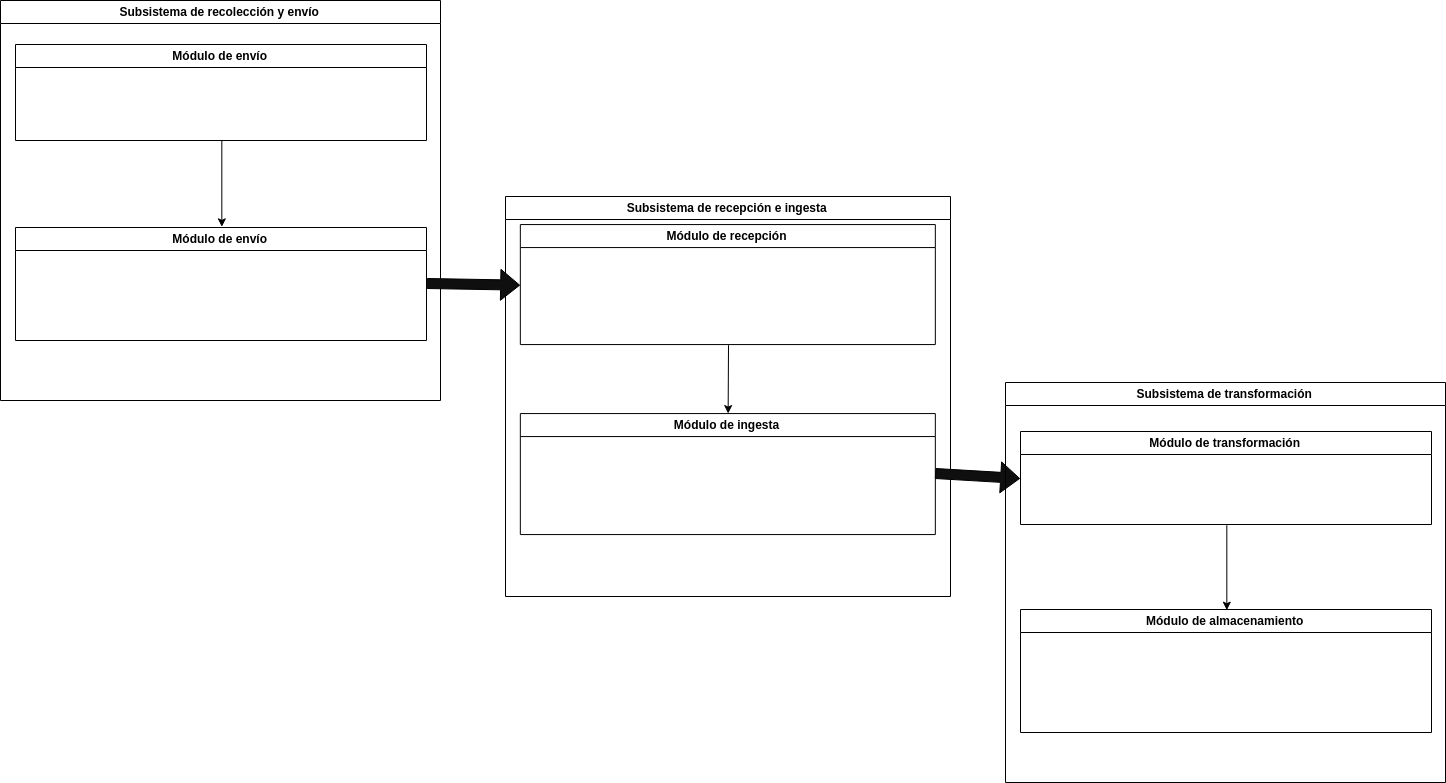
\includegraphics[width=\linewidth] {Moduloss-arquitecturaparcial.png}
	\caption{Vista parcial de la arquitectura del sistema}
	\label{fig:arqparcial}
\end{figure}

La arquitectura del sistema se divide en tres partes o subsistemas, cada subsistema tiene una tarea diferenciada dentro del sistema. En la figura \ref{fig:arqparcial} se puede ver una vista parcial de como se relacionan los subsistemas y los módulos del sistema. Las flechas indican el sentido del flujo de datos.
 
 
 Los subsistemas son los siguientes:

\begin{itemize}
	\item \textit{Subsistema de recolección y envío}: Está compuesto de dos módulos, el de recolección y el de envío. El módulo de recolección se encarga de recoger los eventos en el dispositivo ubicuo. El módulo de envío se encarga de enviar los eventos recogidos por el módulo de recolección al módulo de recepción del subsistema de recepción e ingesta.
	
	\item \textit{Subsistema de recepción e ingesta}: Está compuesto por dos módulos, el de recepción y el de ingesta. El módulo de recepción se encarga de centralizar la ingesta de eventos a un único punto de entrada y  de recibir los eventos que le envía el módulo de envío. El módulo de ingesta se encarga de recibir los eventos del módulo de recepción y almacenarlos como mínimo hasta que el módulo de transformación los consuma.

	\item \textit{Subsistema de transformación}:  Está compuesto por dos módulos, el de transformación y el de almacenamiento. El módulo de transformación se encarga de transformar los eventos que consume del módulo de ingesta y de enviarlos al módulo de almacenamiento. El módulo de almacenamiento recibe los eventos transformados del módulo de transformación y los almacena.
\end{itemize}

La arquitectura propuesta cumple con las fases del proceso ETL. Los encargados de la Extracción son el subsistema de recolección y envío, y el subsistema de recepción e ingesta. El encargado de la Transformación y la Carga es el subsistema de transformación.

Esta arquitectura está basada en la arquitectura Kappa\cite{Tfg:kappa}, siendo el módulo de ingesta el que implemente la capa de almacenamiento de datos, el módulo de transformación el que implemente la capa de Stream Processing y el módulo de almacenamiento el que implemente la capa en la cual se sirven los datos.


\chapter{Subsistema de recolección y envío}

\section{Arquitectura del subsistema}

\begin{figure}[!htb]
	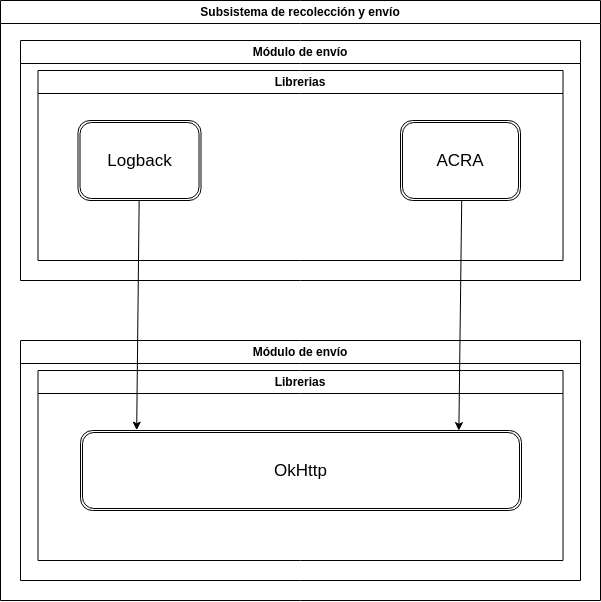
\includegraphics[width=\linewidth]{Moduloss-subrecenv.png}
	\caption{Vista general del subsistema de recolección y envío}
	\label{fig:subrecenv}
\end{figure}

El subsistema de recolección y envío está formado por dos módulos, los cuales actúan en el dispositivo ubicuo. Esta es una división a nivel lógico y existe para reducir a problemas más simples el problema general, aunque nada impide que una herramienta implemente dos módulos. En la figura \ref{fig:subrecenv} se puede ver como se relacionan los módulos y las herramientas del subsistema. Las flechas indican el sentido del flujo de datos.

\subsection{Módulo de recolección}
El módulo de recolección es el encargado de recoger los eventos en el dispositivo ubicuo, para que luego el módulo de envío pueda consumirlos. 
\\\\
En concreto para este proyecto los eventos que se recogen son logs y crashlogs. Los logs servirán para llevar a cabo la monitorización y los crashlogs el seguimiento de errores.
\\\\
Para generar logs se han de explicitar en el código ahí donde el programador considere adecuado, los crashlogs se generan automáticamente cuando la aplicación termina inesperadamente.
\\\\
Los logs se recolectan en tiempo de ejecución y se almacenan en el dispositivo ubicuo para que el módulo de envío los consuma cuando sea pertinente.
\\\\
Los crashlogs se recolectan cuando la aplicación termina inesperadamente y no se almacenan en el dispositivo, sino que de forma inmediata el módulo de envío los consume. Se ha decidido que no se almacenen en el dispositivo puesto que, se considera que tienen más prioridad que los logs, y porque no se puede asegurar que se lleguen a almacenar en el dispositivo o que la aplicación pueda volverse a abrir después de que el crash haya sucedido. Así pues se invoca directamente al módulo de envío para que consuma tal crashlog.

\subsection{Módulo de envío}
El módulo de envío es el encargado de consumir los eventos que ha recolectado el módulo de recolección y enviar tales eventos al módulo de recepción del subsistema de recepción e ingesta.
\\\\
El envío de los logs lo hace cuando la aplicación se cierra correctamente. Es entonces cuando consume los logs almacenados en el dispositivo y los envía al módulo de recepción.
\\\\
El envío de los crashlogs lo hace cuando la aplicación se ha cerrado inesperadamente. Es entonces cuando consume el crash generado y lo envía al módulo de recepción.

\section{Estructura del sistema}

\subsection{Módulo de recolección}
El módulo de recolección está integrado por dos librerías. Una librería se encarga de recolectar los logs y otra los crashlogs.
\\\\
La librería encargada de recolectar logs como mínimo ha de permitir que el programador defina logs en el punto del programa donde este considere oportuno, y que se pueda definir el destino de los logs.

La librería encargada de recolectar crashlogs como mínimo ha de identificar cuando se ha producido un cierre inesperado de la aplicación, recuperar el error que ha notificado el sistema sobre el cierre inesperado, formar un crashlog con la información recopilada y permitir definir el destino del crashlog.

\subsection{Módulo de envío}
El módulo de envío está integrado por una librería. Esta librería se encarga de enviar los logs y los crashlogs recolectados mediantes peticiones HTTP. Como mínimo esta librería ha de poder formar una petición HTTP conteniendo los eventos recolectados, y enviarla a un destino.

\section{Herramientas utilizadas}

Las herramientas utilizadas para llevar a cabo los módulos han sido librerías para Android.

\subsection{Módulo de recolección}
Para llevar a cabo la recolección de logs se ha utilizado la librería Logback\cite{Tfg:logbackandroid} en su versión para Android. Esta librería permite definir en que punto del programa se quiere generar un log y redirigir la salida del log a diferentes destinos. Esta librería también nos permite editar el formato de salida del log así como la metainformación que se añade al log.

Para llevar a cabo la recolección de crashlogs se ha utilizado la librería ACRA\cite{Tfg:acra}. Esta librería detecta cuando una aplicación ha acabado inesperadamente y genera un crashlog con información de valor para reconocer que puede haber pasado. Esta librería también permite redirigir la salida del crashlog a diferentes destinos, editar el formato de salida del crashlog y la metainformación que se añade al crashlog.

\subsection{Módulo de envío}
Para llevar a cabo el envío de logs y crashlogs se ha utilizado la librería OkHttp\cite{Tfg:okhttp} que permite hacer peticiones HTTP\cite{Tfg:HTTPv1-1}. Se ha escogido esta librería por la rapidez con la que se puede programar lo que se desea para este proyecto, a parte del uso eficiente que hace de los recursos del sistema.

\section{Configuración del subsistema}

\subsection{Módulo de recolección}


Del módulo de recolección se han configurado los siguientes factores:

\subsubsection{Metadatos}
Metadatos hace referencia a toda la información que se recolecta a parte de la información de valor del evento. La información de valor n el caso de los logs es el mensaje de define el programador, en el caso de los crashlogs es el mensaje de error del crash.

De los los logs se recogen metadatos porque se consideran útiles para entender el contexto del log, los metadatos que se recogen son:

\begin{itemize}	
	\item \textbf{Hora del evento}: Hora en la que se produce el evento
	\item \textbf{Tiempo que transcurre desde que se inició la aplicación}: Una resta entre la hora que se produce el evento y la hora que se inició la aplicación.
	\item \textbf{Nivel}: Los logs pueden tener varios niveles, nivel informativo, de debug, de error, y más niveles que se pueden definir.
	\item \textbf{Nombre del thread}: Nombre del thread que lanza el log para que sea recolectado.
\end{itemize}

De los los crashlogs se recogen metadatos porque se consideran útiles para entender el contexto del crashlog y poder solucionar el error cuanto antes, los metadatos que se recogen son:

\begin{itemize}
	\item Versión de la aplicación
	\item Modelo del dispositivo
	\item RAM total del dispositivo
	\item RAM disponible en el momento del crash
	\item Versión de Android
	\item Tipo de CPU
	\item Tipos de CPU soportadas por el dispositivo
\end{itemize}

\subsubsection{Formato}
El formato escogido para representar tanto logs, como crashlogs ha sido un objeto JSON puesto que nos aporta el poder tratar el evento de manera fácil y para cumplir con los requisitos de formato que exige el módulo de recepción. Cada dato que se quiere incluir en el evento es un par clave-valor, donde la clave es fija y el valor depende del estado del dispositivo. Las claves de los crahslogs no se han podido definir, sino que ACRA define las que han de ser. En el caso de los logs sí que se han podido definir, para reducir el uso de red y de almacenamiento estas claves son tan solo un carácter, el módulo de transformación se configurará para que sea capaz de enriquecer los logs y de reconocer que significa cada carácter. 

\subsubsection{Destino}
Destino hace referencia a donde se envían los eventos una vez se han recolectado. 
Los logs no pasan directamente al módulo de envío, sino que se almacenan en un archivo de texto en el dispositivo ubicuo para que cuando la aplicación se cierre, el módulo de envío los consuma de ese archivo.
Los crashlogs pasan directamente a disposición del módulo de envío una vez se recolectan. No se almacenan en persistencia. 

\subsection{Módulo de envío}

Del módulo de envío se han configurado los siguiente factores:

\begin{itemize}
	\item \textbf{Cuándo se hace el envío}: En el caso de los logs, el envío se hace una vez la aplicación se ha cerrado, se hace así para no interferir en el uso de red mientras la aplicación está corriendo. En Android es posible detectar cuando se va a cerrar una aplicación y ejecutar código. \\ En el caso de los crashlogs el envío se hace justo cuando el crash sucede, se hace así ya que nada asegura que la aplicación pueda volverse a abrir después de que un crash haya sucedido. La librería ACRA nos permite llevar a cabo este comportamiento con los crashlogs.
	
	\item \textbf{Destino}: El destino tanto de los logs como de los crashlogs es el módulo de recepción, por lo que se ha configurado para que sean enviados ahí. Dentro del módulo de ingesta, logs y crashlogs van a destinos lógicos diferentes, por lo que también se ha configurado su destino dentro del módulo de ingesta.
	
	\item \textbf{Cómo se hace el envío}: En el caso de crashlogs no hay más opción a que cada petición HTTP POST hacía el módulo de recepción contenga tan solo un crashlog. En el caso de los logs se puede enviar una petición HTTP POST por cada log o envíar una petición HTTP POST con todos los logs recolectados durante la sesión. Se ha escogido enviar una sola petición HTTP POST con todos los logs recolectados para no saturar al módulo de recepción atendiendo peticiones.
\end{itemize}



















\chapter{Subsistema de recepción e ingesta}

\section{Arquitectuta del subsistema}

\subsection{Módulo de recepción}

El módulo de recepción en el encargado de recibir los eventos módulo de envío y de enviárselos al módulo de ingesta. Por lo que este módulo no almacena de forma persistente los eventos recibidos.
\\\\
Se ha añadido un módulo entre el módulo de envío y el módulo de ingesta para centralizar a un punto de entrada y una metodología de envío universales a todos los dispositivos ubicuos de la empresa. De esta manera también, se facilita el que nuevos dispositivos ubicuos, diferentes a los que la empresa utiliza, puedan integrarse con el sistema.

\subsection{Módulo de ingesta}

El módulo de ingesta es el encargado de recibir los eventos del módulo de recepción y dejar a disposición los datos al módulo de transformación para que este los consuma. Por lo que este módulo almacena de forma persistente los eventos recibidos.
\\\\
Se ha añadido un módulo entre el módulo de recepción y el módulo de transformación por dos razones:

\begin{enumerate}
	\item No saturar al módulo de transformación.
	\item No perder eventos si el módulo de transformación está caído.
\end{enumerate}

Puesto que el módulo de ingesta sirve los datos para que sean consumidos, el módulo de transformación los consume cuando pueda consumirlos, de esta manera si estaba caído, y puesto que módulo de ingesta almacena los datos de forma persistente, los consumirá una vez esté otra vez arriba.


\section{Infraestructura del subsistema}

\subsection{Módulo de recepción}
El módulo de recepción lo integra una API REST que sea capaz de recibir los eventos y enviarlos al módulo de ingesta. Se ha escogido una API REST, puesto 

\subsection{Módulo de ingesta}
El módulo de ingesta lo integra una streaming platform, una especie de buffer, que es capaz de recibir los eventos y almacenarlos en disco hasta que el módulo de transformación los consuma.


\section{Herramientas utilizadas}

\subsection{Módulo de recepción}
Kafka Rest Proxy\cite{Tfg:kafkarestproxy}

\subsection{Módulo de ingesta}
Apache Kafka\cite{Tfg:kafka}



\chapter{Subsistema de transformación}

\section{Arquitectura del subsistema}

El subsistema de transformación está formado por dos módulos, los cuales actúan fuera del dispositivo ubicuo. Esta es una división a nivel lógico y existe para reducir a problemas más simples el problema general, aunque nada impide que una herramienta implemente dos módulos.

\subsection{Módulo de transformación}

El módulo de transformación es el encargado de consumir los datos del módulo de ingesta, hacer las transformaciones deseadas a los datos y publicarlas en el módulo de almacenamiento. Este módulo no almacena de forma persistente los datos.

Este módulo es necesario ya que nos ayuda a crear información de valor con los eventos extraídos, a parte de generar la información en un formato que el módulo de almacenamiento acepte.

\subsection{Módulo de almacenamiento}

El módulo de almacenamiento es el encargado de recibir los datos transformados del módulo de transformación y almacenarlos para que puedan ser consumidos por otros sistemas o aplicaciones.

Este módulo es necesario ya que es el encargado de almacenar de forma persistente los datos transformados y sin él otros sistemas no podrían consumir los datos transformados.


\section{Estructura del subsistema}

La estructura de este subsistema puede variar mucho dependiendo de los datos que se quieran procesar, en nuestro casos son logs y crashlogs, por lo que la estructura utilizada ha de ser capaz de transformar de forma eficaz logs y crashlogs, pero la elección de la estructura no ha de condicionar el propósito del sistema. Aunque el sistema del proyecto ha de trabajar con eventos, se ha buscado la solución más general para tener lo más cercano a un sistema de propósito general, de esta manera se podrán procesar otro tipo de datos cuando sea necesario. Se ha de tener en cuenta que la elección del módulo de almacenamiento no se ha tomado en este proyecto, sino que este sistema se ha tenido que acoplar con un módulo de almacenamiento existente en la empresa, por lo que la elección estructural del módulo de transformación se ha visto en parte condicionada por el módulo de almacenamiento existente.


\subsection{Módulo de transformación}

Para el módulo de transformación se ha buscado por un lado, que sea eficaz transformando logs y crashlogs y por otro que sea lo más general posible para soportar en el futuro la transformación de otro tipo de datos, por lo que la solución encontrada pasa por aprovechar la existencia de un módulo de ingesta extremadamente versátil y dividir en submódulos, que pueden colaborar entre ellos, el módulo de transformación. Así pues, los elementos a nivel estructural han de encajar en esta división.
\\\\
El módulo de transformación se divide en dos submódulos:

\subsubsection{Submódulo de propósito general}

El submódulo de propósito general es capaz de transformar todo tipo de datos, ya sean eventos u otra cosa. Este submódulo se ha añadido para dotar al sistema de generalidad transformando datos. Este submódulo es capaz de hacer agregaciones, joins y windowing en tiempo real. A parte, este submódulo es fácilmente escalable, desplegable e integrable con el submódulo de ingesta. La solución escogida ha sido, en vez de una estructura pasiva a la que se le envían lotes de trabajo para que los procese, un solución activa en la que una aplicación con el uso de alguna librería sea capaz de consumir los datos del módulo de ingesta, transformarlo, y publicarlos en el módulo de almacenamiento. Por lo que a nivel estructural este submódulo es una aplicación que utiliza una librería de stream processing.

\subsubsection{Submódulo de propósito específico}
El submódulo de propósito específico es capaz de transformar un tipo de datos en concreto, en el caso de este proyecto eventos. Este módulo hace transformaciones que requieren una potencia de cálculo menor que las transformaciones que puede hacer el submódulo de propósito general. Las transformación que principalmente efectúa es un enriquecimiento para que los datos sean aceptados en el módulo de destino o para que el submódulo de propósito general haga transformaciones más potentes con los datos ya enriquecidos. \\\\

%% !!!si tienes uno de caracter especifico pasivo uno de caracter general activo, el de caracter general es escalable y adaptable. Tienes un módulo específico potente y uno general ligeramente menos potente que la media pero mucho más barato, por lo que los dos submódulos se complementan para dar un sistema escalable y versatil.

Es decir, este módulo delega en el submódulo de transformación de propósito general cuando ha de hacer transformaciones potentes.

\subsection{Módulo de almacenamiento}
El módulo de almacenamiento nos venía dado por la empresa. La empresa ya utilizaba un módulo de almacenamiento en concreto y el sistema se ha de integrar con él. El módulo de almacenamiento lo integra una aplicación de seguimiento de errores y un servidor de búsqueda. Los dos elementos tienen bases de datos, pero para acceder a ellas se ha de hacer a través de los puntos de entrada que disponen, API REST por ejemplo. El sistema se ha de integrar con este módulo.
\section{Herramientas utilizadas}

\subsection{Módulo de transformación}
\subsubsection{Submódulo de propósito general}
Para el submódulo de propósito general se ha decidido utilizar Kafka Streams\cite{Tfg:kafkastreams}
%%Kafka streams
\subsubsection{Submódulo de propósito específico}
%%Logstash
\subsection{Módulo de almacenamiento}
%%Elastic Search, JIRA

\section{Configuración del subsistema}



\chapter{Visión completa de la arquitectura del sistema}

En la figura \ref{fig:arqfinal} se puede ver como se relacionan los subsistemas, los módulos y las herramientas del sistema. Las flechas finas indican el sentido del flujo de datos entre módulos del mismo subsistema, las flechas gruesas indican el flujo de datos entre subsistemas. Las flechas entre Logstash, Kafka Streams y Apache Kafka son bidireccionales ya que tanto Logstash como Kafka Streams pueden utilizar Apache Kafka como buffer para hacer cálculos parciales. 

\begin{figure}[!htb]
	
	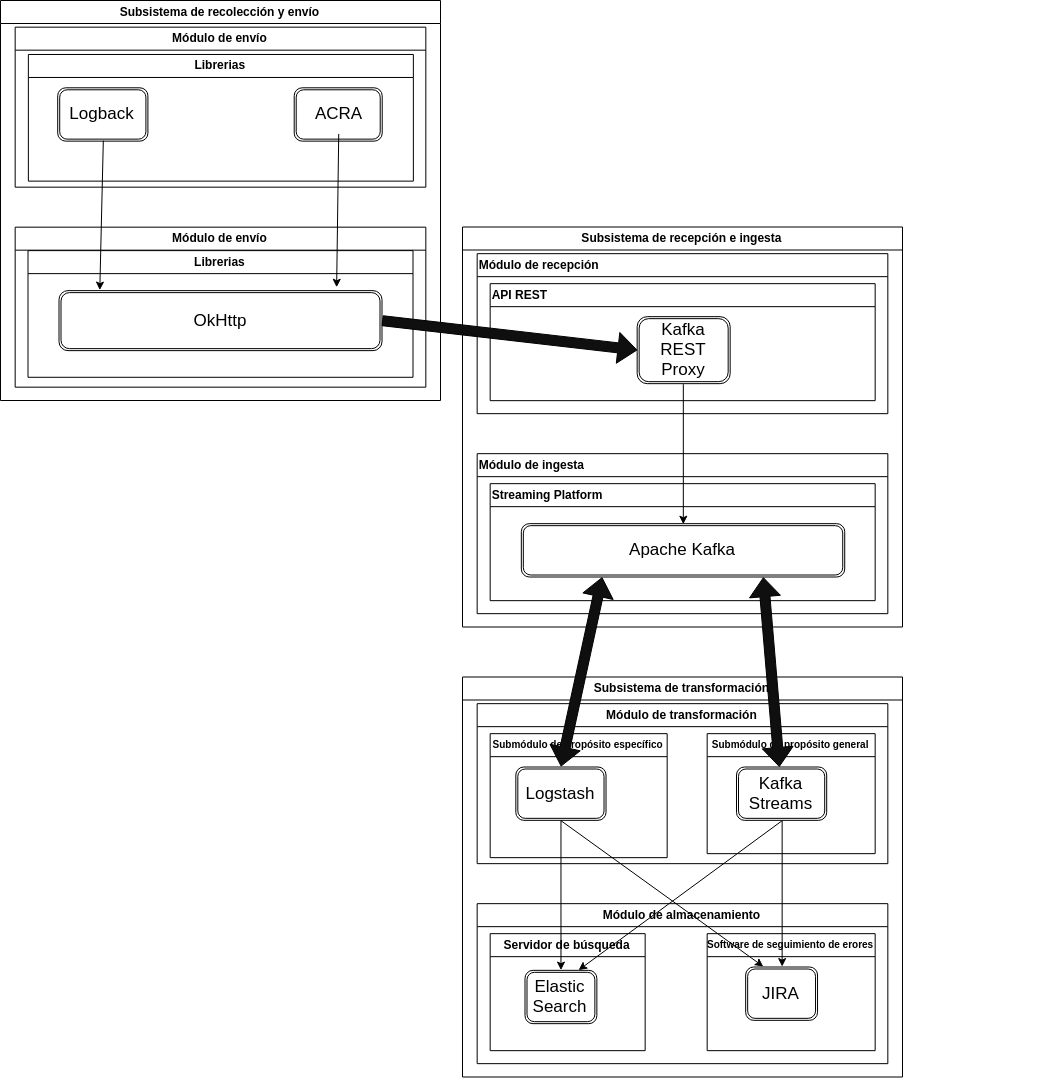
\includegraphics[width=\linewidth] {Moduloss-estructura-todos.png}
	\caption{Visión general de la arquitectura del sistema}
	\label{fig:arqfinal}
\end{figure}
\chapter{Despliegue} \label{cap:despligue}
\section{Entorno}
El entorno que se ha escogido para desplegar las partes del sistema que no residen en el dispositivo ubicuo ha sido Amazon Web Services (AWS)\footnote{\href{https://aws.amazon.com}{https://aws.amazon.com}}. La razón es porque la empresa actualmente trabaja con este servicio y es más fácil integrarse con los módulos con los que se ha de integrar el sistema. AWS nos ofrece una serie de servicios que encajan con lo que se pretende desplegar.

El entorno que se ha escogido para desplegar las partes del sistema que residen en el dispositivo ubicuo ha sido Android. La razón es porque la empresa trabaja actualmente con dispositivos Android y tenía la necesidad de recolectar eventos en estos dispositivos.

\section{Máquinas}
El servicio que se ha escogido para desplegar las máquinas ha sido EC2\cite{Tfg:ec2}, ya que ofrece diferentes máquinas virtuales con diferentes características a nivel de hardware que pueden adaptarse notablemente a las necesidades de las diferentes partes del sistema.

\subsection{Subsistema de recolección y envío}
Para desplegar este subsistema tan solo se necesita un dispositivo Android. La versión mínima de Android ha de ser la 4.0 para que las librerías funcionen correctamente. El dispositivo ha de tener acceso a Internet para que pueda comunicarse con el subsistema de recepción e ingesta.

\subsection{Subsistema de recepción e ingesta}
\subsubsection{Módulo de recepción}
Este módulo hace un uso intensivo de CPU y red\cite{Tfg:restproxykafka}. El uso de red es elevado, puesto que ha de ser capaz de soportar diversas conexiones concurrentes en las cuales se pueden transmitir gran cantidad de datos. El uso de CPU es intensivo ya que cada petición POST la atiende un thread. Kafka Rest Proxy explota el paralelismo de la CPU, a más cores, más peticiones podrá atender. El uso de RAM que hace este módulo es modesto y con que pueda soportar 1GB de heap es suficiente. El uso de disco es mínimo, ya que no almacena ninguna información en ellos.
\\

La máquina escogida para desplegar este módulo ha sido la c5.2xlarge, en la tabla \ref{tabla:c5.2xlarge} se pueden ver sus recursos hardware.


\begin{table}[H]\label{tabla:c5.2xlarge}
	\centering
	\begin{tabular}{|l|l|}
		\hline
		\textbf{Máquina}            & \textbf{c5.2xlarge}    \\ \hline
		\textbf{CPUs}               & 8 cores                \\ \hline
		\textbf{RAM}                & 16.0 GiB               \\ \hline
		\textbf{Rendimiento de red} & Hasta 10 Gbps          \\ \hline
		\textbf{HDD tamaño}         & 30 GiB                 \\ \hline
		\textbf{HDD IOPS máximos}   & 3000 IOPS              \\ \hline
	\end{tabular}
	\caption{Recursos hardware de la máquina virtual c5.2xlarge}
\end{table}



Para asegurar la confiabilidad del módulo y de paso aumentar el número de cores del sistema, se ha decidido desplegar 3 máquinas c5.2xlarge y un balanceador de carga que distribuya las conexiones entre las máquinas. Para desplegar el balanceador de carga se ha escogido utilizar el servicio que presta AWS de Aplication Load Balancer\cite{Tfg:apploadbalancer}.
\\
Con tal despliegue se puede soportar que caigan dos máquinas y aún el módulo podrá continuar haciendo su trabajo. Si ninguna máquina está caída se tendrán 24 cores y se podrán soportar conexiones de hasta 30 Gbps de tráfico agregado.

%%Foto

\subsubsection{Módulo de ingesta}
Este módulo hace un uso intensivo de RAM, red y disco. Para que Apache Kafka pueda funcionar necesita un orquestador que dirija y balancee los diferentes nodos (brokers) de Apache Kafka. Este orquestador es Apache Zookeeper. Apache Kafka y Apache Zookeeper hacen un uso diferente de los recursos, para no sobredimensionar las máquinas y reducir costes, Kafka y Zookeeper se desplegarán en máquinas con diferentes recursos.
\\\\
El uso que hace Kafka de los recursos es el siguiente\cite{Tfg:kafkadeploy}:

\begin{itemize} 
	\item \textbf{CPU}: Hace un uso ligero de CPU, si se ha de elegir entre CPUs rápidas o con muchos cores, mejor una con muchos cores.
	\item \textbf{RAM}: Hace un uso intensivo de RAM, menos de 16 GB es improductivo.
	\item \textbf{Red}: Hace un uso intensivo de red, menos de 1 GbE es improductivo.
	\item \textbf{HDD}: Hace un uso intensivo de disco, se necesita espacio dependiendo del volumen de datos a tratar y un throughput elevado.
\end{itemize}

El uso que hace Zookeeper de los recursos es el siguiente\cite{Tfg:zookeeperdeploy}:

\begin{itemize} 
	\item \textbf{CPU}: Hace un uso ligero de CPU.
	\item \textbf{RAM}: Hace un uso ligero de RAM, menos de 8 GB es improductivo.
	\item \textbf{Red}: Hace un uso intensivo de red, menos de 1 GbE es improductivo.
	\item \textbf{HDD}: Hace un uso intensivo de disco, se necesita un throughput elevado.
\end{itemize}

Con tales premisas, la máquina escogida para desplegar Apache Kafka ha sido la r4.xlarge, en la tabla \ref{tabla:kafkazookeeper} se pueden ver sus recursos hardware. La máquina escogida para desplegar Apache Zookeeper ha sido la r4.large, en la tabla \ref{tabla:c5.2xlarge} se pueden ver sus recursos hardware.

\begin{table}[H]\label{tabla:kafkazookeeper}
	\centering
	\begin{tabular}{|l|l|l|}
		\hline
		\textbf{Máquina}            & \textbf{r4.large} & \textbf{r4.xlarge} \\ \hline
		\textbf{CPUs}               & 2 cores           & 4 cores            \\ \hline
		\textbf{RAM}                & 15.25 GiB         & 30.5 GiB           \\ \hline
		\textbf{Rendimiento de red} & Hasta 10 Gbps     & Hasta 10 Gbps      \\ \hline
		\textbf{HDD tamaño}         & 30 GiB            & 500 GiB            \\ \hline
		\textbf{HDD IOPS máximos}   & 3000 IOPS         & 3000 IOPS          \\ \hline
	\end{tabular}
	\caption{Recursos hardware de la máquina virtual r4.large y r4.xlarge}
\end{table}

Zookeeper necesita un mínimo de 3 máquinas para funcionar, por lo que se han desplegado 3 máquinas r4.large.
Kafka no tiene un número mínimo de máquinas para funcionar, pero para aumentar la confiabilidad, la durabilidad y el rendimiento, se han desplegado 3 máquinas r4.xlarge.

\subsection{Subsistema de transformación}
El despliegue del subsistema de transformación es particular puesto que un módulo ya está desplegado en la empresa. Para dar completud al trabajo, en aquellos módulos que ya estén desplegados, se hablará de las máquinas que se desplegarán para hacer la demostración el día de la lectura del trabajo.

\subsubsection{Módulo de transformación}
Al estar dividido el módulo de transformación en dos submódulos y encargarse de tareas diferentes, el uso de los recursos es diferente en los dos submódulos. 
\\
Para el submódulo de propósito específico se ha desplegar Logstash, en la documentación de la herramienta no se deja del todo claro los requerimientos hardware\cite{Tfg:logstashdeploy}, pero por su naturaleza se ha supuesto que hace un uso intensivo de CPU, RAM y red, y un uso ligero de disco. De momento se ha desplegado en una r4.xlarge, en la tabla \ref{tabla:kafkazookeeper} se puede ver sus recursos hardware. Como trabajo futuro, se ha monitorear el rendimiento de este submódulo para ver el uso de los recursos que hace, y cambiar si fuera necesario la máquina utilizada.
\\
Para el submódulo de propósito general se ha de desplegar la aplicación Java que utiliza Kafka Streams. El despliegue de máquinas para este submódulo depende mucho del volumen de datos que se hayan de procesar, para la demostración se va a suponer un volumen de datos pequeño, tan solo para verificar que la solución funciona. La máquina escogida es una t2.micro en la tabla \ref{tabla:t2.micro} se pueden ver sus recursos hardware.

\begin{table}[H]\label{tabla:t2.micro}
	\centering
	\begin{tabular}{|l|l|}
		\hline
		\textbf{Máquina}            & \textbf{t2.micro}      \\ \hline
		\textbf{CPUs}               & 1 cores                \\ \hline
		\textbf{RAM}                & 1.0 GiB                \\ \hline
		\textbf{Rendimiento de red} & Moderado               \\ \hline
		\textbf{HDD tamaño}         & 30 GiB                 \\ \hline
		\textbf{HDD IOPS máximos}   & 3000 IOPS              \\ \hline
	\end{tabular}
	\caption{Recursos hardware de la máquina virtual t2.micro}
\end{table}

Se van a desplegar 3 máquinas r4.xlarge para el submódulo de propósito específico, con el objetivo de distribuir la carga entre los servidores y aumentar la potencia de procesado.
\\
Se va a desplegar 1 máquina t2.micro para el submódulo de propósito general, con el objetivo de comprobar la solución propuesta.

\subsection{Módulo de almacenamiento}
Este módulo ya está desplegado en la empresa, por lo que el despliegue que se ha hecho es exclusivo para la demostración. Por un lado se ha desplegado un cluster de Elastic Search y una máquina con Kibana, y por otro una máquina con JIRA.

Para el despliegue del cluster de Elastic Search se han utilizado máquinas parecidas a las que utiliza la empresa. La máquina escogida es una r4.xlarge, en la tabla \ref{tabla:kafkazookeeper} se puede ver sus recursos hardware. Para el despligue de Kibana se ha utilizado una t2.micro, ya que JIRA no consume grandes recursos, en la tabla \ref{tabla:t2.micro} se puede ver los recursos hardware de la máquina escogida.
\\
Para el despligue de JIRA se va a utilizar una t2.small ya que JIRA como mínimo requiere 2 GiB de RAM para funcionar fluido. En la tabla \ref{tabla:t2.small} se puede ver los recursos hardware de la máquina escogida.

\begin{table}[H]\label{tabla:t2.small}
	\centering
	\begin{tabular}{|l|l|}
		\hline
		\textbf{Máquina}            & \textbf{t2.small}      \\ \hline
		\textbf{CPUs}               & 1 cores                \\ \hline
		\textbf{RAM}                & 2.0 GiB                \\ \hline
		\textbf{Rendimiento de red} & Moderado               \\ \hline
		\textbf{HDD tamaño}         & 30 GiB                 \\ \hline
		\textbf{HDD IOPS máximos}   & 3000 IOPS              \\ \hline
	\end{tabular}
	\caption{Recursos hardware de la máquina virtual t2.small}
\end{table}

Se van a desplegar 3 máquinas r4.xlarge para Elastic Search ya que se quiere comprobar el correcto funcionamiento del sistema cuando Elastic Search está distribuido en más de una máquina. Se va desplegar 1 máquina t2.micro para Kibana. Se va a desplegar una máquina t2.small para JIRA.

\subsection{Resumen de servicios a desplegar}

\begin{table}[H]\label{tabla:resumenservicios}
	\centering
	\resizebox{15cm}{!}{
	\begin{tabular}{|l|l|l|l|l|}
		\hline
		\textbf{Módulo} & \textbf{Aplicación} & \textbf{Servicio}      & \textbf{Detalle}          & \textbf{Número} \\ \hline
		Recepción       & Kafka Rest Proxy    & Amazon EC2             & c5.2xlarge                & 3               \\ \hline
		Recepción       & Kafka Rest Proxy    & Elastic Load Balancing & Application Load Balancer & 1               \\ \hline
		Ingesta         & Apache Kafka        & Amazon EC2             & r4.xlarge                 & 3               \\ \hline
		Ingesta         & Apache Zookeeper    & Amazon EC2             & r4.large                  & 3               \\ \hline
		Transformación  & Logstash            & Amazon EC2             & r4.xlarge                 & 3               \\ \hline
		Transformación  & Kafka Streams       & Amazon EC2             & t2.micro                  & 1               \\ \hline
		Almacenamiento  & Elastic Search      & Amazon EC2             & r4.xlarge                 & 3               \\ \hline
		Almacenamiento  & Kibana              & Amazon EC2             & t2.micro                  & 1               \\ \hline
		Almacenamiento  & JIRA                & Amazon EC2             & t2.small                  & 1               \\ \hline
	\end{tabular}
    }
	\caption{Recursos de servicios a desplegar}
\end{table}

En la tabla \ref{tabla:resumenservicios} se pueden ver el resumen de los servicios a desplegar en AWS. La columna \textit{Módulo} nos dice el módulo del sistema que se despliega, la columna \textit{Aplicación} nos marca la aplicación que se va a desplegar, la columna \textit{Servicio} no dice el servicio de AWS que se va a utilizar, la columna \textit{Detalle} nos informa sobre que servicio en concreto se va a desplegar y la columna \textit{Número} no dice el número de instancias que se van a desplegar. Cada fila corresponde a los servicios a desplegar.

\subsection{Vista general del despliegue}\label{cap:networking}

\begin{figure}[!htb]
	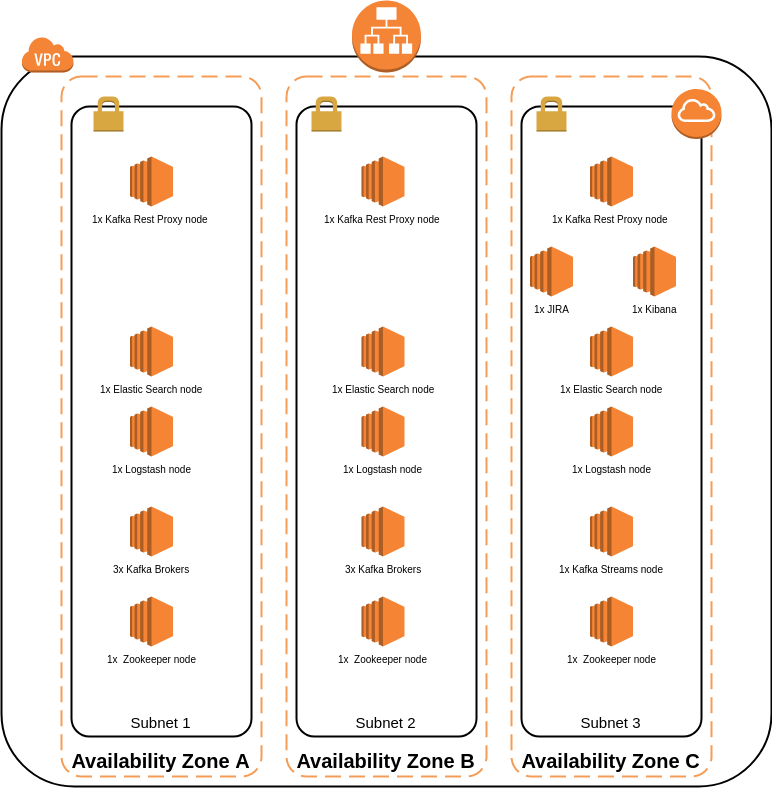
\includegraphics[width=\linewidth] {Moduloss-netdeploy.png}
	\caption{Networking del despliegue en AWS}
	\label{fig:networking1}
\end{figure}

En la figura \ref{fig:networking1} se puede ver el como queda el despliegue de red de las máquinas, y una leyenda con el significado de los iconos. Para interconectar las diferentes máquinas, AWS son ofrece el servicio Amazon Virtual Private Cloud (Amazon VPC), esta VPC es una red virtual que interconecta las máquinas virtuales que se han desplegado, funciona igual que una red local tradicional. En la figura \ref{fig:networking1} se puede ver como existen 3 subredes que residen en 3 Availability Zones diferentes. AWS trabaja con los conceptos de región y zonas de disponibilidad. La VPC reside en una región, una región es una porción geográfica de un país. Las zonas de disponibilidad son diferentes data centers dentro de la región. En el caso de la figura, el sistema reside en una zona y está disperso entre los diferentes data centers de la zona. Se ha hecho así para aumentar la confiabilidad del sistema ya que tal y como se han configurado los diferentes módulos, el sistema es tolerante a caídas de servidores, y desplegarlos en diferentes zonas de disponibilidad disminuye la posibilidad de que caigan dos máquinas a la vez del mismo módulo.
\\\\
La figura \ref{fig:networking1} también muestra que la VPC está encabezada por un Aplication Load Balancer, este balanceador de carga es el que recibe las peticiones del dispositivo ubicuo y distribuye la carga entre los 3 Kafka Rest Proxy nodes. Por último, la figura muestra en la Subnet 3 una Internet Gateway, se ha añadido para que las máquinas de JIRA y de Kibana sean accesibles desde Internet.



%%Problematicas
\chapter{Metodología y rigor}
\section{Método de trabajo}
Se ha utilizado un modelo de desarrollo en cascada \cite{Tfg:waterfall}, ya que es una planificación sencilla, fácil de entender y utilizar por alguien que no está acostumbrado a trabajar siguiendo un método concreto. Para el éxito de este proyecto y utilizando esta metodología, es muy importante la documentación, cosa que es positiva ya que este proyecto luego será utilizado en una empresa y ayudará a que los desarrolladores de la empresa tengan referencias e información sobre diferentes aspectos del proyecto. Al tener desde un principio la mayoría de requisitos del proyecto definidos, era poco probable que surgieran necesidades imprevistas, esto sumado al hecho de que el desarrollo del proyecto lo ha llevado a cabo una única persona y por lo tanto no ha tenido que sincronizarse con otros trabajadores, ha hecho que el modelo cascada sea uno de los más adecuados para este proyecto.

A parte del uso del modelo de desarrollo cascada, la comunicación con el director del trabajo ha sido frecuente, ya sea para hablar de aspectos generales del proyecto, o de aspectos más concretos. La comunicación ha sido vía email o en persona. Se pactaron reuniones con el director cada quince días para comprobar los avances del proyecto. 

\section{Herramientas de seguimiento}
Para el seguimiento del desarrollo del software se ha utilizado el sistema de control de versiones Git y estas versiones se almacenan en un repositorio remoto, se ha utilizado GitHub como repositorio remoto.

Para el seguimiento del diseño e implementación del sistema se ha generado documentación que se publicará en el JIRA de la empresa. Para asegurar que el diseño y la implementación es aparentemente correcta se ha consultará con el director antes de publicar la documentación en JIRA.

Para la generación de documentación de seguimiento se ha utilizado la suite ofimática LibreOffice, también LaTeX y se publicará en JIRA bajo el formato PDF.

\section{Métodos de validación}

Los métodos de validación corresponderían a la fase de validación del desarrollo en cascada.

La parte de implementación del proyecto se puede dividir en las siguientes fases:

\begin{itemize}
	\item Subsistema de recolección y envío de eventos
	\item Subsistema de recepción e ingesta de eventos
	\item Subsistema de transformación de eventos
	\item Integración con JIRA y ES Stack
\end{itemize}

Se ha aplicado el desarrollo en cascada de forma independiente en cada fase del proyecto por lo que se obtienen cuatro fases de validación.

\subsection{Validación del subsistema de recolección y envío}
La fase de validación del subsistema de recolección y envío de eventos consiste en la creación de una sencilla aplicación que integra las librerías escogidas en la fase de diseño con el fin de que recolecte y envíe eventos a un servidor desplegado en un entorno de pruebas. Tal servidor consiste en una máquina virtual que simula ser el subsistema de recepción e ingesta de eventos. Se ha modificado todo aquello de la aplicación que era erróneo hasta que se ha conseguido el resultado esperado en el servidor. Una vez se ha conseguido el resultado esperado, se han exportado las configuraciones a los entornos de producción.

%%Foto de la app del movil con el nombre TFG recolección y envío

En la Figura \ref{fig:android} se puede ver una captura de la aplicación que se ha creado para validar que se recogen y envían los eventos correctamente. Consiste en dos botones, uno que genera un crash y otro que genera un log con el texto que se le ponga en la textbox. Luego la aplicación, en el caso del crash lo envía al módulo de recepción sin almacenarlo en el dispositivo, y en el caso del log lo almacena en el dispositivo hasta que lo envía cuando la aplicación se cierra.

\begin{figure}[!htb]
	\centering
	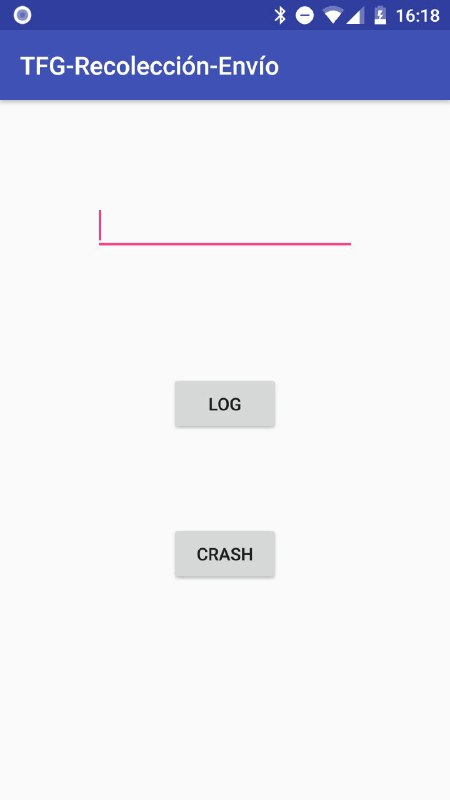
\includegraphics[scale=0.40] {captura.jpeg}
	\caption{Captura de la aplicación de validación}
	\label{fig:android}
\end{figure}

\subsection{Validación del subistema de recepción e ingesta}
La fase de validación del subistema de recepción e ingesta de eventos consiste en, por un lado configurar en una máquina virtual el módulo de recepción para que sea capaz de recibir eventos y pasarlos al módulo de ingesta. Por otro lado se ha de configurar en otra máquina virtual el módulo de ingesta de eventos para que sea capaz de comunicarse con el módulo de recepción de eventos y almacenar de forma parcial los eventos. Una vez las dos máquinas virtuales se comuniquen entre si, y los mensajes enviados al módulo de recepción se almacenen en el módulo de ingesta, se ha considerado que la configuración principal era la correcta y se ha procedido a exportar tal configuración al entorno de producción.

%%Foto con output de la petición POST y foto con output del topic logs y crashes


En la Figura \ref{fig:POST} se puede ver la respuesta positiva que da el módulo de recepción a la petición HTTP POST para publicar datos en el módulo de ingesta. El código 200 de HTTP indica que el comportamiento es esperado. A parte del código 200, se ofrece información sobre como se han distribuido los datos en el módulo de ingesta, cosa que ayuda a validar el módulo de ingesta, en la Figura \ref{fig:POST} se puede ver tal información.

\begin{figure}[!htb]
	\centering
	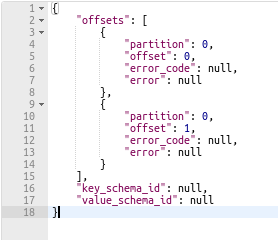
\includegraphics[scale=0.60] {kafka-rest.png}
	\caption{Cuerpo de la respuesta HTTP del módulo de recepción}
	\label{fig:POST}
\end{figure}


En la Figura \ref{fig:logs} se ve el contenido del topic logs y en la Figura \ref{fig:crashes} el contenido del topic crashes. Si los logs y los crashes que se generan con la aplicación aparecen en sus respectivos topics es que tanto el módulo de recepción como el de ingesta están funcionando correctamente.

\begin{figure}[!htb]
	\centering
	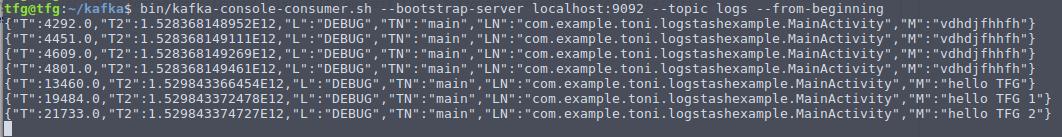
\includegraphics[scale=0.60, width=\linewidth] {kafka-logs.png}
	\caption{Contenido del topic logs}
	\label{fig:logs}
\end{figure}


\begin{figure}[!htb]
	\centering
	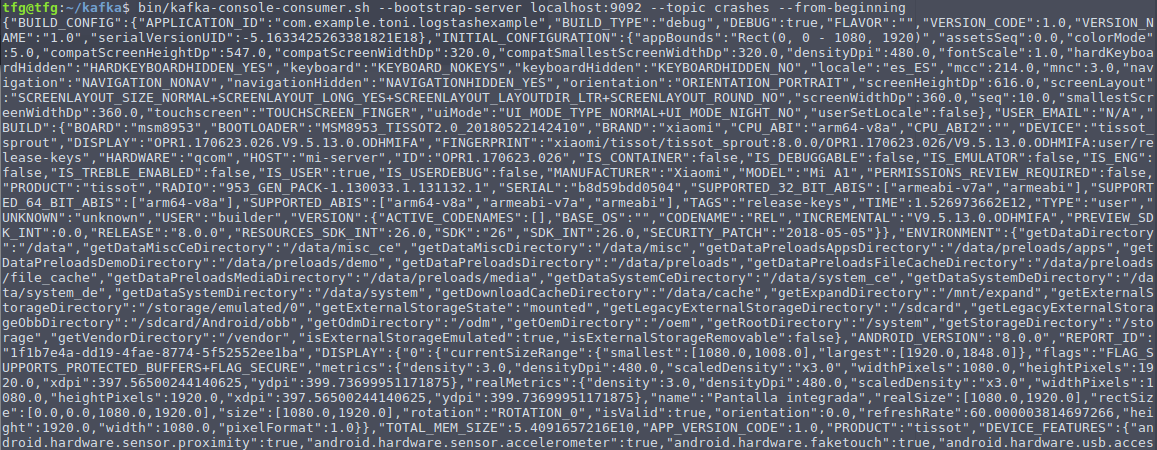
\includegraphics[scale=0.60, width=\linewidth] {kafka-crashes.png}
	\caption{Contenido del topic crashes}
	\label{fig:crashes}
\end{figure}

\subsection{Validación del subsistema de transformación}
La fase de validación del subsistema de transformación de eventos, consiste en lanzar las aplicaciones de procesado y configurar en local una máquina virtual con el subsistema de recepción e ingesta de eventos a la cual se han ido enviando eventos, tales eventos van a ser consumidos por la aplicación de procesado que se ha programado y por Logstash, se ha redirigido la salida de tales aplicaciones a la consola para validar que la transformación es la correcta, una vez se han obtenido los datos esperados, se ha procedido a desplegar las configuraciones en entornos de producción.

%%Foto output kafka streams logstash

En la Figura \ref{fig:crashout} se puede ver el resultado de la transformación de Kafka Streams, el formato del mensaje es el esperado, por lo que se puede dar por validado.

\begin{figure}[!htb]
	\centering
	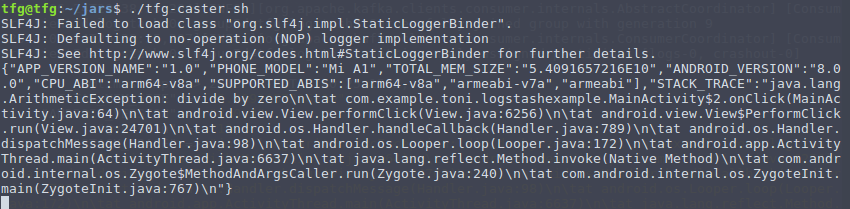
\includegraphics[scale=0.60, width=\linewidth] {crashout.png}
	\caption{Resultado de la transformación con Kafka Streams}
	\label{fig:crashout}
\end{figure}

En la Figura \ref{fig:logstash} se ve como queda el mensaje una vez ha sido transformado por Logstash, como el formato del mensaje es el esperado, se puede dar por validado.

\begin{figure}[!htb]
	\centering
	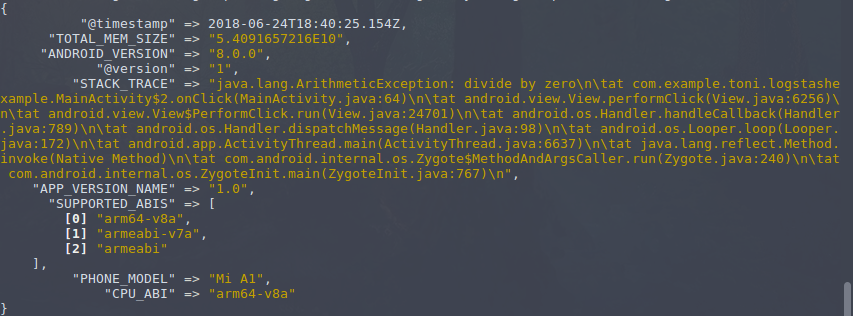
\includegraphics[scale=0.60, width=\linewidth] {logstash.png}
	\caption{Resultado de la transformación con Logstash}
	\label{fig:logstash}
\end{figure}




\subsection{Validación de la integración con JIRA y ELK Stack}
La fase de validación de la integración con JIRA y ELK Stack consiste en montar en local los tres subsistemas, un nodo con JIRA y un nodo con toda la ELK Stack, refinar las configuraciones de los módulos hasta que se consiga, recolectar, enviar, recibir, ingerir, transformar y cargar un evento en JIRA y en la ELK Stack. En JIRA se tendrá que generar un ticket con información sobre el evento. En ls ELK Stack, Logstash ya ha hecho una transformación del evento, lo pasará a Elastic Search, y Kibana será capaz de consumir el evento apuntando a Elastic Search. Una vez se ha conseguido el comportamiento deseado, se han exportado las configuraciones a los entornos de producción.

En la Figura \ref{fig:jira} se puede ver el ticket en JIRA que se ha creado fruto de los crashes que se han generado.

\begin{figure}[H]
	\centering
	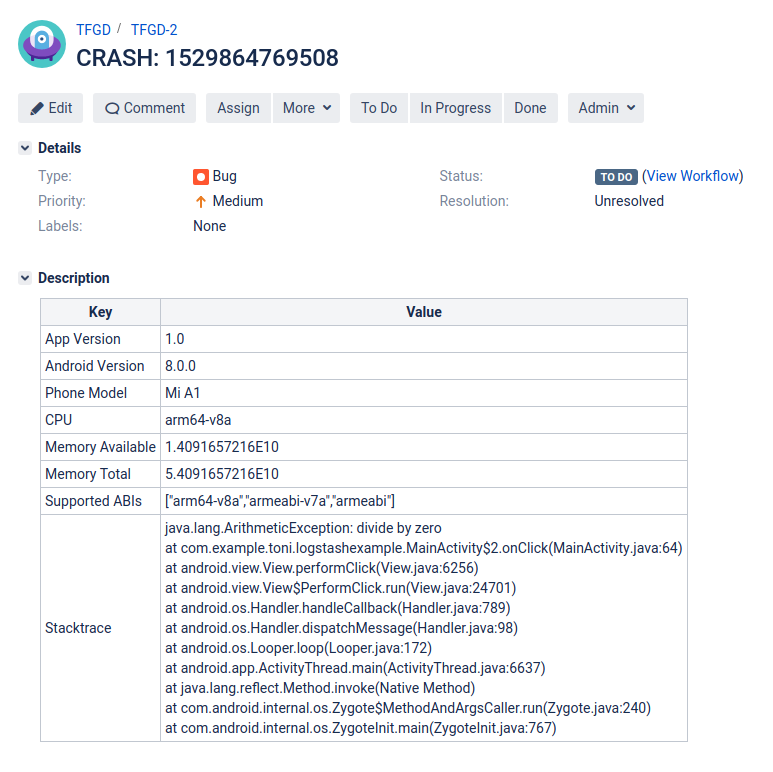
\includegraphics[scale=0.4] {jira.png}
	\caption{Ticket resultante en JIRA}
	\label{fig:jira}
\end{figure}

En la Figura \ref{fig:kibana} se ve diferentes resultados en Kibana que se han creado fruto de los eventos que se han generado.

\begin{figure}[H]
	\centering
	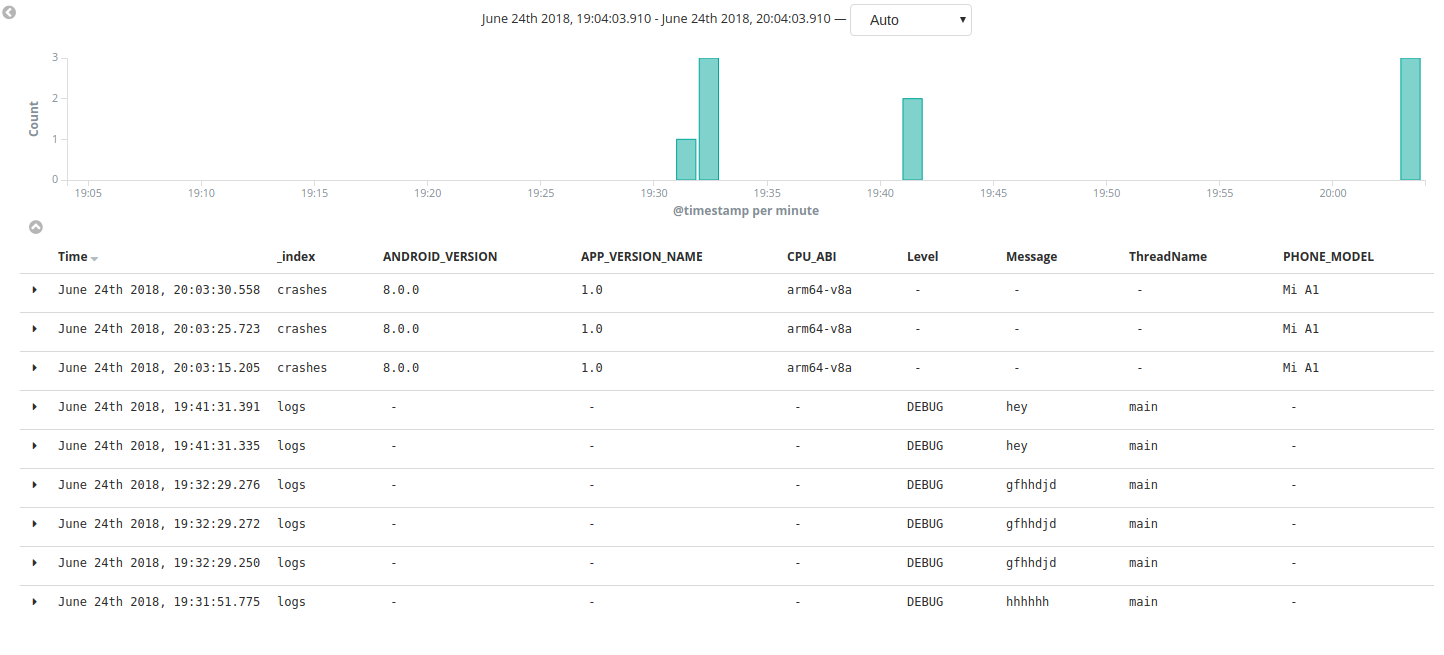
\includegraphics[scale=0.5, width=\linewidth] {kibana.png}
	\caption{Resultados generados por los eventos}
	\label{fig:kibana}
\end{figure}

Puesto que el ticket en JIRA existe, y los resultados en Kibana también, significa que todos los módulos del sistema funcionan correctamente y se puede dar por validado la totalidad el sistema.

Una vez han estado todos los módulos corriendo en producción, también se ha testeado que se cumpla el comportamiento esperado. Para ello se han generado una serie de eventos, los cuales han de seguir el pipeline hasta llegar a JIRA y Kibana. Cuando JIRA y Kibana han mostrado lo deseado se ha concluido el testeo.

Además de tales pruebas y para asegurar el correcto avance del diseño del proyecto, se ha mantenido un contacto frecuente con el director para que vaya dando su visto bueno. Todas las pruebas y tests las ha llevado a cabo el desarrollador del proyecto.
\chapter{Planificación final}\label{cap:planificacion}
\section{Cambios en la planificación inicial y en la gestión económica}

Respecto la planificación inicial han habido cambios en la duración del proyecto, ha pasado de durar 540 horas a 420 horas en total. Esta reducción de horas ha sido debida a que la dificultad con la que se había previsto algunas fases del proyecto ha sido menor. Las fases que han reducido sus horas son las siguientes:

\begin{itemize}
	\item \textbf{Subsistema de recolección y envío de eventos} de 90 horas a 66 puesto que la integración de las librerías se ha llevado a cabo sin muchas complicaciones.
	
	\item \textbf{Subsistema de transformación de eventos} de 90 horas a 60 puesto que las herramientas con las que se ha desarrollado dicha transformación no tenían una curva de aprendizaje tan pronunciada como la que se previó.
	
	\item \textbf{Integración con JIRA y ES Stack} de 90 horas a 30 puesto que tanto JIRA como ES están pensados para que su integración sea rápida y fácil.
	
	\item \textbf{Despliegue del sistema} de 18 horas a 6 horas puesto que la mayoría de elementos ya se habían desplegado en las fases anteriores.
	
	\item \textbf{Testeo del sistema en producción} de 18 a 12 horas puesto que gran parte de las pruebas ya se habían realizado en las fases anteriores.
\end{itemize}

La tarea \textit{Integración con JIRA y ES Stack} en el plan inicial tan solo era \textit{Integración con JIRA}, en la planificación final también ha habido una integración con ES Stack.

La reducción de tiempo del proyecto también repercute positivamente en el coste del proyecto, ya que gran parte del coste va ligado a las horas de proyecto. Aunque se cometió un fallo en el cálculo del presupuesto inicial, esta reducción de horas, más la corrección de dicho error ha hecho que el coste total del proyecto disminuya de 33.499,55 € a 24.297,26 €.

En los capítulos \ref{cap:planificacion} y \ref{cap:gestionec} se expone la nueva planificación y los nuevos presupuestos contando esta reducción de horas. En el Anexo \ref{cap:ganttanex} se encuentra el diagrama de Gantt definitivo en la Figura \ref{fig:gantt}, así como el diagrama de Gantt que se planteó al inicio en la Figura \ref{fig:ganttini}.


\section{Tabla de tiempo}
En el Tabla \ref{tabla:tiempotareas} se muestran, de forma definitiva, las tareas a realizadas y el tiempo que se ha empleado para realizar tales tareas, en la Sección \ref{cap:gantt} se especificarán con más detalle.

\begin{table}[H]\label{tabla:tiempotareas}
	\centering
	\begin{tabular}{|l|l|l|}
		\hline
		\textbf{Tarea}                               & \textbf{Horas previstas} & \textbf{Horas empleadas}       \\ \hline
		Aprendizaje                                  & 150 horas                & \textbf{150 horas}             \\ \hline
		Subsistema de recolección y envío de eventos & 90 horas                 & \textbf{66 horas}              \\ \hline
		Subsistema de recepción e ingesta de eventos & 90 horas                 & \textbf{90 horas}              \\ \hline
		Subsistema de transformación de eventos      & 90 horas                 & \textbf{60 horas}              \\ \hline
		Integración con JIRA y ES Stack              & 90 horas                 & \textbf{30 horas}              \\ \hline
		Despliegue del sistema                       & 15 horas                 & \textbf{6 horas}               \\ \hline
		Testeo del sistema en producción             & 15 horas                 & \textbf{12 horas}              \\ \hline
		\textbf{Horas totales del proyecto}          & 540 horas                & \underline{\textbf{420 horas}} \\ \hline
	\end{tabular}
	\caption{Tiempo de realización de las tareas}
\end{table}

\section{Restricciones}
Las restricciones no han cambiado con respecto las restricciones del plan inicial que se encuentran en la Sección \ref{sec:restriccionesini} del Capítulo \ref{cap:planini}.

\section{Recursos}
\subsection{Recursos humanos}
Se ha dispuesto de un desarrollador que es quién ha llevado a cabo el proyecto. El desarrollador de este proyecto ha asumido las tareas de jefe de proyecto, consultor y Site Reliability Engineer (SRE) \cite{Tfg:sre}. El tiempo en horas por semana que ha dedicado el desarrollador al proyecto ha sido de 30 horas por semana. Es una medida aproximada ya que ha variado por la influencia de diversos factores tales como la carga de trabajo que tenga ha tenido desarrollador por causas externas al proyecto.

También se ha dispuesto de un director, el cual podrá ha sido consultado por el desarrollador.

\subsection{Recursos físicos}\label{cap:recfis}
\begin{description}

	\item [Lenovo Y700] Computadora donde se ha desarrollado el proyecto y se han hecho las pruebas parciales antes de desplegar el sistema. Se ha utilizado también para escribir la memoria.
	
	\item [Xiaomi MI A1] Celular con el que se han hecho las pruebas de recolección y envío de eventos.
	
	\item [GitHub] Servidor remoto de control de versiones. Se ha utilizado para almacenar las diferentes versiones del software que se ha desarrollado.
	
	\item [JIRA] Herramienta para administración de tareas de un proyecto. Se publicará documentación de los diversos módulos en ella.
	
	\item [Servidores de producción] En la Sección \ref{sec:presrechard} se especifican las máquinas necesarias así como el coste de utilizarlas.
\end{description}

\section{Diagrama de Gantt}\label{cap:gantt}
En el Anexo \ref{cap:ganttanex} se encuentra el diagrama de Gantt final (Figura \ref{fig:gantt}) donde se especifican cada una de las tareas, su fecha de inicio y fin, su duración en horas y el coordinador o responsable de cada tarea. Se ven también las restricciones temporales de cada tarea.

Las tareas marcadas en rojo indican un riesgo alto a que causen posibles desviaciones.
Las tareas marcadas en azul un riesgo medio a que causen posibles desviaciones.

Las tareas marcadas en verde marcan las reuniones de seguimiento con el director, el espacio temporal entre ellas es de quince días de media, estas reuniones empiezan después de la fase de aprendizaje y duran hasta la semana anterior de la entrega del proyecto. En tales reuniones se ha ido revisando aspectos claves del desarrollo del proyecto así como resolviendo posibles dudas.








\chapter{Gestión económica final}\label{cap:gestionec}
\section{Gastos directos}
\subsection{Presupuesto recursos humanos}
El desarrollador de este proyecto ha asumido las tareas de jefe de proyecto, consultor y Site Reliability Engineer (SRE) \cite{Tfg:sre}. Aún siendo así, los cálculos están hechos basados en precios actuales de mercado y diferenciando cada rol. En el Tabla \ref{tab:preprechum} se ven tales cálculos.

Con relación a las tareas expuestas en el diagrama de Gantt \ref{fig:gantt} de \ref{cap:ganttanex}, al jefe de proyecto le corresponden las tareas de aprendizaje (GEP también está incluido en esta tarea), al consultor le corresponden las tareas de delimitación y al SRE las restantes.


\begin{table}[H]\label{tab:preprechum}
	\centering
	\begin{tabular}{|l|l|l|l|}
		\hline
		\textbf{Rol}              & \textbf{Horas} & \textbf{Precio por hora}         & \textbf{Precio total}  \\ \hline
		\textbf{Jefe de proyecto} & 192 h          & 27 €/h \cite{Tfg:projectmanager} & 5.184 €                \\ \hline
		\textbf{Consultor}        & 42 h           & 20 €/h \cite{Tfg:itconsultant}   & 840 €                  \\ \hline
		\textbf{SRE}              & 258 h          & 34 €/h \cite{Tfg:sresalary}      & 8.772 €                \\ \hline
		\multicolumn{3}{|l|}{\textbf{Total}} & \textbf{\underline{14.796 €}}                                   \\ \hline
	\end{tabular}
	\caption{Presupuesto recursos humanos}
\end{table}


\textbf{\underline{Presupuesto total recursos humanos = 14.796 €}}

\subsection{Presupuesto recursos hardware}\label{sec:presrechard}
Para llevar a cabo el proyecto y como se mostraba en la sección \ref{cap:recfis}, se han utilizado una serie de recursos físicos. En el caso del hardware se han utilizado cuatro elementos, la computadora Lenovo Y700, el celular Xiaomi MI A1, el servidor remoto GitHub y los servidores de producción. 

Es interesante comentar que para los servidores de producción se ha utilizado Amazon Web Service (AWS) \cite{Tfg:aws}, por lo que no se paga por la adquisición de los servidores sino por su uso por hora, se ha supuesto para hacer los cálculos que durante el desarrollo del proyecto se han utilizado todas las horas. No se contará nada más a parte de su coste por horas. Como el precio es bajo demanda, no se ha calculado el tiempo de amortización de los servidores de producción ya que el coste del hardware por hora real ya es el que se paga. 

En el Tabla \ref{tab:prepaws} se muestran las máquinas a utilizar con el gasto total contando que están siempre encendidas a partir de la etapa Desarrollo del sistema.

\begin{table}[H]\label{tab:prepaws}
	\centering
	\begin{tabular}{|l|l|l|l|l|}
		\hline
		\textbf{Instancia}  & \textbf{Número de instancias} & \textbf{Precio por hora} & \textbf{Horas} & \textbf{Precio total} \\ \hline
		\textbf{r4.xlarge}  & 6                             & 0,21 €/h \cite{Tfg:ec2price} & 270 h          & 342,9 €               \\ \hline
		\textbf{r4.large}   & 3                             & 0,12 €/h \cite{Tfg:ec2price} & 270 h          & 97,2 €                \\ \hline
		\textbf{c5.2xlarge} & 3                             & 0,33 €/h \cite{Tfg:ec2price} & 270 h          & 267,3 €               \\ \hline
		\textbf{t2.micro}   & 1                             & 0,01 €/h \cite{Tfg:ec2price} & 270 h          & 2,7 €                 \\ \hline
		\multicolumn{4}{|l|}{\textbf{Total}} & \textbf{\underline{710,1 €}}                                                   \\ \hline
	\end{tabular}
	\caption{Presupuesto AWS}
\end{table}

En el caso de GitHub, se ha utilizado la capa gratuita, por lo que tampoco se ha calculado la amortización.

En el Tabla \ref{tab:preprechw} se muestra el presupuesto final de los recursos hardware con el cálculo de la amortización. Para calcular la amortización en la Tabla \ref{tab:preprechw} como en la Tabla \ref{tab:preprecsw} se han hechos los siguientes supuestos y utilizado la siguiente fórmula:

\label{eq:amortizacion}
\begin{align*}
Amortización = Hp * \frac{Pp}{Av*365*Hd} \\
Hp = Horas \; del \; duración \; del \; proyecto. \\
Pp = Precio \; del \; producto. \\
Av = Años \; de \; vida \; útil \; del \; producto. \\
Hd = Horas \; al \; día \; que \; se \; utiliza \; el \; producto \; (suponemos \; siempre \; 8h). \\
\end{align*}

\begin{table}[H]\label{tab:preprechw}
	\centering
	\begin{tabular}{|l|l|l|l|l|}
		\hline
		\textbf{Producto}               & \textbf{Unidades} & \textbf{Precio} & \textbf{Vida} & \textbf{Amortización} \\ \hline
		\textbf{Lenovo Y700}            & 1                 & 1.099 € \cite{Tfg:ideapad} & 3 años        & 52,69 €               \\ \hline
		\textbf{Xiaomi MI A1}           & 1                 & 229 € \cite{Tfg:mia1}      & 3 años        & 10,98 €               \\ \hline
		\textbf{GitHub}                 & -                 & 0 €             & -             & 0 €                   \\ \hline
		\textbf{Servidores producción}  & -                 & 710,1 €         & -             & 710,1 €               \\ \hline
		\multicolumn{4}{|l|}{\textbf{Total}} & \textbf{\underline{773,77 €}}                                        \\ \hline
	\end{tabular}
	\caption{Presupuesto recursos hardware}
\end{table}

\textbf{\underline{Presupuesto total recursos hardware = 773,77 €}}

\subsection{Presupuesto recursos software}
El único software del que se ha tenido que pagar licencia es JIRA, necesario para la tarea Integración con JIRA y Elastic Search del diagrama de Gantt de la sección \ref{cap:gantt}. La licencia que se va a comprar es una en que nosotros hemos de almacenar JIRA en servidores propios de la empresa y pueden utilizar el software hasta 10 personas. En la Tabla \ref{tab:preprecsw} se muestra el cálculo del presupuesto de los recursos software.

\begin{table}[H]\label{tab:preprecsw}
	\centering
	\begin{tabular}{|l|l|l|l|l|}
		\hline
		\textbf{Producto} & \textbf{Unidades} & \textbf{Precio} & \textbf{Vida} & \textbf{Amortización} \\ \hline
		\textbf{JIRA}     & 1                 & 8 € \cite{Tfg:jiraprice} & 3 años        & 0,38 €                \\ \hline
		\multicolumn{4}{|l|}{\textbf{Total}} & \textbf{\underline{0,38 €}}                               \\ \hline
	\end{tabular}
	\caption{Presupuesto recursos software}
\end{table}

\subsection{Total presupuesto gastos directos}
En la Tabla \ref{tab:preptotal} se muestra el presupuesto total de los gastos directos del proyecto.

\begin{table}[H]\label{tab:preptotal}
	\centering
	\begin{tabular}{|l|l|}
		\hline
		\textbf{Tipo}                          & \textbf{Coste}                   \\ \hline
		\textbf{Presupuesto recursos humanos}  & 14.796 €                         \\ \hline
		\textbf{Presupuesto recursos hardware} & 773,77 €                         \\ \hline
		\textbf{Presupuesto recursos software} &0,38 €                            \\ \hline
		\textbf{Total}                         & \textbf{\underline{15.570,15 €}} \\ \hline
	\end{tabular}
	\caption{Presupuesto total gastos directos}
\end{table}

\section{Gastos Indirectos}\label{sec:gastosin}

Los principales gastos indirectos del proyecto han sido el consumo eléctrico y la conexión a Internet. 

Para el cálculo del consumo eléctrico se han utilizado los siguientes datos:

\begin{itemize}
	\item \textbf{Precio del kWh en España:} 0.10813 €/kWh (Como precio de consumo eléctrico se ha tomado el precio medio del 18 de marzo de 2018 \cite{Tfg:luz} ).
	\item \textbf{Horas de consumo eléctrico:} 420h.
	\item \textbf{Potencia consumida:} 60 + 6*58 = 408 W (Potencia del portátil 60 W, Potencia de los 6 fluorescentes del despacho 58 W).
\end{itemize}

\label{eq:gastoelec}
\begin{align*}
0,408 kW * 420 h * 0,10813 \text{€}/kWh = 18,5 \text{€}
\end{align*}

Para el cálculo de la conexión a Internet se han utilizado los siguientes datos:

\begin{itemize}
	\item \textbf{Precio fibra óptica 100mb Movistar:} 45€/mes.
	\item \textbf{Horas de duración del proyecto:} 420h.
	\item \textbf{1 mes:} 30 días.
	\item \textbf{1 día:} 8h hábiles.
\end{itemize}

\label{eq:costeint}
\begin{align*}
Coste \; de \; Internet = 420h * \frac{45 \text{€}/mes}{30 \; días*8h} = 78,75 \text{€}
\end{align*}

\subsection{Total presupuesto gastos indirectos}

En la Tabla \ref{tab:prepgastosindi} se ve el presupuesto total de los gastos indirectos del proyecto.

\begin{table}[H]\label{tab:prepgastosindi}
	\centering
	\begin{tabular}{|l|l|}
		\hline
		\textbf{Producto}     & \textbf{Coste}                \\ \hline
		\textbf{Electricidad} & 18,5 €                        \\ \hline
		\textbf{Internet}     & 78,75 €                       \\ \hline
		\textbf{Total}        & \textbf{\underline{97,25 €}} \\ \hline
	\end{tabular}
	\caption{Presupuesto total gastos indirectos}
\end{table}

\section{Total presupuesto gastos directos e indirectos}

En la Tabla \ref{tab:preptotaldirindi} se ve el presupuesto total de gastos directos e indirectos del proyecto.

\begin{table}[H]\label{tab:preptotaldirindi}
	\centering
	\begin{tabular}{|l|l|}
		\hline
		\textbf{Tipo}              & \textbf{Coste}                   \\ \hline
		\textbf{Gastos directos}   & 15.570,15 €                      \\ \hline
		\textbf{Gastos indirectos} & 97,25 €                          \\ \hline
		\textbf{Total}             & \textbf{\underline{15.667,40 €}} \\ \hline
	\end{tabular}
	\caption{Presupuesto total de gastos directos e indirectos}
\end{table}

\section{Contingencia}
Dado que el desarrollador del proyecto es la primera vez que se ha enfrentado a muchas de las tecnologías utilizadas para el desarrollo del proyecto y aunque las tareas están bien detalladas, se ha destinado un 20\% del valor total del presupuesto a contingencia. En la Tabla \ref{tab:contingencia} se muestra lo que supone esta contingencia.

\begin{table}[H]\label{tab:contingencia}
	\centering
	\begin{tabular}{|l|l|}
		\hline
		\textbf{Contingencia} & \textbf{Total}                  \\ \hline
		20\%                  & \textbf{\underline{3.133,48 €}} \\ \hline
	\end{tabular}
	\caption{Calculo de contingencia}
\end{table}

\section{Control de gestión}
Se han localizado dos posibles imprevistos, su solución y el gasto que supondrían. A parte de los dos imprevistos encontrados, podrían ocurrir otros, pero ninguna de ellos supondría un gasto de recursos hardware. El gasto extra a nivel de recursos humanos ya se ha contemplado en la Tabla \ref{tab:imprevistos} y el gasto a nivel de software sería nulo ya que se buscarían alternativas gratuitas si hiciera falta. La Tabla \ref{tab:imprevistos} muestra con que porcentaje pueden ocurrir los imprevistos y el impacto económico para el proyecto.

\begin{table}[H]\label{tab:imprevistos}
	\centering
	\begin{tabular}{|l|l|l|l|l|}
		\hline
		Imprevisto                           & Solución   & Probabilidad     & Coste    & Coste total \\ \hline
		Avería del equipo                    & Solución 1 & 10 \%            & 1.099 €  & 109,9 €     \\ \hline
		Retraso de alguna fase del proyecto  & Solución 2 & 10 \%            & 11.696 € & 1.169,6 €   \\ \hline
		\multicolumn{4}{|l|}{\textbf{Total}} & \textbf{\underline{1.279,5 €}}                         \\ \hline
		                                                                        
	\end{tabular}
	\caption{Imprevistos del proyecto}
\end{table}

\textbf{Solución 1}: Comprar otro similar

\textbf{Solución 2}: Aumento de las horas trabajadas por el SRE (8h/día). No se recalcula el coste de luz para facilitar los cálculos.

\section{Coste total}

En la Tabla \ref{tab:totaltotal} se ve el presupuesto del coste total del proyecto. El total con IVA es de \textbf{\underline{24.297,26 €}}

\begin{table}[H]\label{tab:totaltotal}
	\centering
	\begin{tabular}{|l|l|l|}
		\hline
		\multirow{4}{*}{}    & \textbf{Tipo}                 & \textbf{Coste}       \\ \hline
		& Directo e indirecto   & 15.667,40 € \\ \hline
		& Contingencia          & 3.133,48 €  \\ \hline
		& Imprevistos           & 1.279,5 €   \\ \hline
		\multicolumn{2}{|l|}{\textbf{Total sin IVA}}            & 20.080,38 € \\ \hline
		\multicolumn{2}{|l|}{\textbf{Total con el 21\% de IVA}} & \textbf{\underline{24.297,26 €}} \\ \hline
	\end{tabular}
    \caption{Coste total del proyecto}
\end{table}





\chapter{Identificación de leyes y regulaciones}

Las dos normativas a las cuales este proyecto podría ser sensible de recibir la aplicación es la Ley Orgánica de Protección de Datos de Carácter Personal (LOPD) a nivel estatal y el Reglamento General de Protección de Datos (GDPR) a nivel europeo, pero no a tal proyecto no se le aplican dichas normativas puesto que no se están recogiendo los datos que tales leyes consideran como sensibles.

La LOPD considera datos de carácter personal: cualquier información numérica, alfabética, gráfica, fotográfica, acústica o de cualquier otro tipo concerniente a personas físicas identificadas o identificables.
En ningún caso se está recogiendo información que puede hacer al usuario identificable.

El GDPR considera datos personales todos aquellos que puedan revelar la identidad del usuario. También incluye direcciones IP pero en el presente proyecto no se recogen direcciones IP de los usuarios.
\chapter{Sostenibilidad}
\section{Impacto económico}
En la Sección 7 se ha estimado el coste para la realización del proyecto. Al ser una previsión de costes se ha sido generoso redondeando ciertos precios y haciendo ciertas estimaciones. Por lo que el coste final del proyecto podrá variar y se espera que varíe a menos, ya que por ejemplo, la estimación de costes de los recursos humanos se ha hecho con el sueldo correspondiente a cada rol cuando en realidad en este proyecto no es así, pero se ha querido enfocar de esta manera para tener una previsión parecida que la que tendría la competencia. 

Siguiendo con la comparación con la competencia, los costes para este proyecto aún inflando los precios son más bajos que los de la competencia ya que las necesidades y los recursos también son más bajos. El hecho de que se plantee el problema de forma diferente que las demás compañías puede hacer que la necesidad de recursos sea menor y este hecho puede ser el que sea mejor a las soluciones existentes a nivel económico, ya que se está diseñando un sistema desde cero en vez de adaptar una solución concreta para que resuelva un problema similar al que ya soluciona. Como resultado se es más eficiente a la hora de adquirir servidores y servicios.

\section{Impacto ambiental}
El indicador de impacto ambiental de este proyecto es principalmente el consumo eléctrico. En la sección 7.2 se ha detallado el consumo eléctrico de la realización del proyecto, en el momento en que el proyecto pase a producción, el consumo eléctrico ya no dependerá íntegramente de la empresa. Se planteó el hecho de comprar servidores y colocarlos en la empresa en vez de alquilar por horas los servidores, esta idea se desestimó y una de las razones fue el consumo eléctrico. AWS es una empresa especializada en el alquiler de servidores y como tal busca su máximo beneficio, por lo que AWS intentará disminuir al máximo su consumo eléctrico dado que reduciendo el consumo aumentan sus beneficios. Por lo tanto, con AWS se está seguro de que se tiene el mínimo consumo eléctrico y por ende el mínimo impacto ambiental.
El proyecto se ha diseñado en vistas a que pueda ser utilizado para procesar otro tipo de datos diferente a los eventos, como pudiera ser los derivados del BI, por lo que ya en el planteamiento inicial del proyecto se pensó en reutilizar recursos a posteriori, a priori no se han podido reutilizar recursos dado que no existían. 
Actualmente las empresas que se disponen a procesar eventos tienden a unificar su capa de eventos con su capa de BI, algo muy parecido que lo que intenta este proyecto. La peculiaridad de este proyecto es el hecho de que primero se diseña un sistema para procesar eventos que luego tendrá que soportar procesar datos de BI, cuando las otras empresas plantearon, por diversas razones, el problema isómero, es decir, diseñaron un sistema de procesado de BI que luego están adaptando para procesar eventos. El hecho de no adaptar ningún sistema, sino diseñar un sistema que admita el procesado de los dos tipos de datos puede eliminar ciertos sobrecostes, como máquinas extras resultado de la adaptación y no de un diseño inteligente. Por lo que esta solución puede ser mejor ambientalmente que las existentes dado que se pueden reducir el uso de máquinas extras y como consecuencia un menor gasto eléctrico.

\section{Impacto social}
El impacto personal del proyecto con lo poco que llevo de este ya ha sido elevado, ya que documentándome para entender el estado del arte, me he dado cuenta de la cantidad de recursos que se invierten para proyectos parecidos para el mío y el uso que se le puede dar desde el punto de vista del dueño de los datos. Mi proyecto se centra en la recolección de eventos para mejorar la eficiencia del trabajo de los desarrolladores, pero también el sistema tendrá que ser compatible para procesar datos de BI.
Los datos de BI al fin y al cabo lo que están midiendo es el comportamiento del usuario con respecto nuestro producto. Esto me genera ciertos dilemas éticos con respecto el trabajo futuro y cómo ha de evolucionar el proyecto. Es cierto que las empresas del sector suelen avisar de que recolectan datos del uso que se hace de sus productos, pero desde mi punto de vista los usuarios no son conscientes de qué datos se están recolectando ni cómo se están utilizando, las empresas del sector no acaban de asegurar que hacen con tales datos una vez han sido procesados.
Creo que tengo en deber ético de ser lo más transparente posible con el uso que haré de esos datos ya que con la información que se recolecta se está muy cerca de vulnerar una intimidad que los usuarios no saben que tienen. Por lo que algo que puede mejorar socialmente mi solución es la transparencia con respecto a los datos recolectados. Una vez acabado el Trabajo de Fin de Grado, este proyecto continuará por lo que mi deber debería ser también una labor de concienciación una vez el Trabajo de Fin de Grado haya terminado.
Aunque este sistema tiene sus peligros a nivel de privacidad, existe la necesidad de que exista, ya que analizando los eventos podemos mejorar las aplicaciones y corregir, por ejemplo, fallos de seguridad que podrían afectar más gravemente a la privacidad que el propio sistema. Este sistema nos proporciona un gran poder, por lo que conlleva una gran responsabilidad de que su uso sea el correcto y más beneficioso para la sociedad en general.

\section{Matriz de sostenibilidad}
La matriz de sostenibilidad resume los puntos 8.1, 8.2 y 8.3. Los criterios seguidos para determinar las puntuaciones son: cómo se ha llevado a cabo el proyecto, la utilidad del proyecto y los riesgos que puede suponer tal proyecto.
El objetivo intrínseco del proyecto es conseguir un mejor rendimiento de los productos de la empresa para aumentar su beneficio económico, por lo que en la dimensión económica obtiene un 10/10 ya que es viable y se pueden apreciar ciertas mejoras con respecto la competencia. En la dimensión ambiental se ha intentado buscar soluciones que no afecten directamente sobre el medio-ambiente de forma negativa, pero al delegar a otras compañías ciertos servicios del proyecto no se puede estar completamente seguro de cumplan su compromiso ambiental, por lo que la puntuación es 6/10. En la dimensión social existente varios riesgos de impactar negativamente, pero el desarrollador del proyecto se compromete a ser transparente en este aspecto, cosa que puede ser diferencial con la competencia por lo que la puntuación que se obtiene es de 8/10.

\begin{table}[H]
	\centering
	\begin{tabular}{|c|c|c|}
		\hline
		\textbf{Dimensión económica} & \textbf{Dimensión ambiental} & \textbf{Dimensión social}  \\ \hline
		       10/10                 &        6/10                  &       8/10                 \\ \hline
		\multicolumn{3}{|c|}{\textbf{Total 23/30}} \\ \hline
	\end{tabular} 
	\caption{Matriz de sostenibilidad}
\end{table}

\chapter{Conclusiones}

\section{Observaciones}

Realizar este proyecto ha permitido a la empresa disponer de un sistema de seguimiento y monitorización de errores en tiempo real, agilizando así la resolución de problemas críticos en los dispositivos que actúan como clientes. Se han cumplido los objetivos planteados al inicio puesto que la prueba de concepto es funcional y desarrolla el comportamiento esperado.

El sistema se ha puesto en producción en la empresa, después de someterlo a una serie de test de validación, con el objetivo de testear el sistema en el entorno empresarial no en el académico.

A título personal este trabajo me ha servido para adquirir unos nuevos conocimientos sobre las arquitecturas de los sistemas de Big Data, en especial los sistema de Stream Processing. También he adquirido nuevos conocimientos de administración de sistemas en AWS así como administración del networking.

\section{Trabajo futuro}

El sistema cumple con los objetivos planteados al inicio del proyecto, pero para que esté listo en un entorno empresarial le falta pulir algunos aspectos.
Así pues al sistema se le ha de dotar de monitorización en todos sus módulos y de seguridad como mínimo en los módulos que están expuestos a Internet.

Este sistema también ha de servir para recoger eventos de otros dispositivos diferentes a los ubicuos, en este caso se han de adaptar los módulos de recolección y de envío al dispositivo objetivo. A raíz de este hecho, se ha de estudiar que tipo de eventos o métricas se han de extraer en tales dispositivos que nos indiquen su correcto funcionamiento.

Un apecto a largo plazo es el de explotar al máximo las herramientas de la Elastic Search Stack. Se quiere utilizar la herramienta de Machine Learning que ofrece. Esta herramienta de Machine Learning se utilizaría principalmente para identificar más rápidamente los posibles errores en las aplicaciones o los dispositivos y para reducir los falsos positivos.




%%MONITOREAR Y COMPROBAR QUE NO HA HABIDO SOBREDIMENSIONAMIENTO

%%%%%%
%%\chapter{Planificación final}\label{cap:planificacion}
\section{Cambios en la planificación inicial y en la gestión económica}

Respecto la planificación inicial han habido cambios en la duración del proyecto, ha pasado de durar 540 horas a 420 horas en total. Esta reducción de horas ha sido debida a que la dificultad con la que se había previsto algunas fases del proyecto ha sido menor. Las fases que han reducido sus horas son las siguientes:

\begin{itemize}
	\item \textbf{Subsistema de recolección y envío de eventos} de 90 horas a 66 puesto que la integración de las librerías se ha llevado a cabo sin muchas complicaciones.
	
	\item \textbf{Subsistema de transformación de eventos} de 90 horas a 60 puesto que las herramientas con las que se ha desarrollado dicha transformación no tenían una curva de aprendizaje tan pronunciada como la que se previó.
	
	\item \textbf{Integración con JIRA y ES Stack} de 90 horas a 30 puesto que tanto JIRA como ES están pensados para que su integración sea rápida y fácil.
	
	\item \textbf{Despliegue del sistema} de 18 horas a 6 horas puesto que la mayoría de elementos ya se habían desplegado en las fases anteriores.
	
	\item \textbf{Testeo del sistema en producción} de 18 a 12 horas puesto que gran parte de las pruebas ya se habían realizado en las fases anteriores.
\end{itemize}

La tarea \textit{Integración con JIRA y ES Stack} en el plan inicial tan solo era \textit{Integración con JIRA}, en la planificación final también ha habido una integración con ES Stack.

La reducción de tiempo del proyecto también repercute positivamente en el coste del proyecto, ya que gran parte del coste va ligado a las horas de proyecto. Aunque se cometió un fallo en el cálculo del presupuesto inicial, esta reducción de horas, más la corrección de dicho error ha hecho que el coste total del proyecto disminuya de 33.499,55 € a 24.297,26 €.

En los capítulos \ref{cap:planificacion} y \ref{cap:gestionec} se expone la nueva planificación y los nuevos presupuestos contando esta reducción de horas. En el Anexo \ref{cap:ganttanex} se encuentra el diagrama de Gantt definitivo en la Figura \ref{fig:gantt}, así como el diagrama de Gantt que se planteó al inicio en la Figura \ref{fig:ganttini}.


\section{Tabla de tiempo}
En el Tabla \ref{tabla:tiempotareas} se muestran, de forma definitiva, las tareas a realizadas y el tiempo que se ha empleado para realizar tales tareas, en la Sección \ref{cap:gantt} se especificarán con más detalle.

\begin{table}[H]\label{tabla:tiempotareas}
	\centering
	\begin{tabular}{|l|l|l|}
		\hline
		\textbf{Tarea}                               & \textbf{Horas previstas} & \textbf{Horas empleadas}       \\ \hline
		Aprendizaje                                  & 150 horas                & \textbf{150 horas}             \\ \hline
		Subsistema de recolección y envío de eventos & 90 horas                 & \textbf{66 horas}              \\ \hline
		Subsistema de recepción e ingesta de eventos & 90 horas                 & \textbf{90 horas}              \\ \hline
		Subsistema de transformación de eventos      & 90 horas                 & \textbf{60 horas}              \\ \hline
		Integración con JIRA y ES Stack              & 90 horas                 & \textbf{30 horas}              \\ \hline
		Despliegue del sistema                       & 15 horas                 & \textbf{6 horas}               \\ \hline
		Testeo del sistema en producción             & 15 horas                 & \textbf{12 horas}              \\ \hline
		\textbf{Horas totales del proyecto}          & 540 horas                & \underline{\textbf{420 horas}} \\ \hline
	\end{tabular}
	\caption{Tiempo de realización de las tareas}
\end{table}

\section{Restricciones}
Las restricciones no han cambiado con respecto las restricciones del plan inicial que se encuentran en la Sección \ref{sec:restriccionesini} del Capítulo \ref{cap:planini}.

\section{Recursos}
\subsection{Recursos humanos}
Se ha dispuesto de un desarrollador que es quién ha llevado a cabo el proyecto. El desarrollador de este proyecto ha asumido las tareas de jefe de proyecto, consultor y Site Reliability Engineer (SRE) \cite{Tfg:sre}. El tiempo en horas por semana que ha dedicado el desarrollador al proyecto ha sido de 30 horas por semana. Es una medida aproximada ya que ha variado por la influencia de diversos factores tales como la carga de trabajo que tenga ha tenido desarrollador por causas externas al proyecto.

También se ha dispuesto de un director, el cual podrá ha sido consultado por el desarrollador.

\subsection{Recursos físicos}\label{cap:recfis}
\begin{description}

	\item [Lenovo Y700] Computadora donde se ha desarrollado el proyecto y se han hecho las pruebas parciales antes de desplegar el sistema. Se ha utilizado también para escribir la memoria.
	
	\item [Xiaomi MI A1] Celular con el que se han hecho las pruebas de recolección y envío de eventos.
	
	\item [GitHub] Servidor remoto de control de versiones. Se ha utilizado para almacenar las diferentes versiones del software que se ha desarrollado.
	
	\item [JIRA] Herramienta para administración de tareas de un proyecto. Se publicará documentación de los diversos módulos en ella.
	
	\item [Servidores de producción] En la Sección \ref{sec:presrechard} se especifican las máquinas necesarias así como el coste de utilizarlas.
\end{description}

\section{Diagrama de Gantt}\label{cap:gantt}
En el Anexo \ref{cap:ganttanex} se encuentra el diagrama de Gantt final (Figura \ref{fig:gantt}) donde se especifican cada una de las tareas, su fecha de inicio y fin, su duración en horas y el coordinador o responsable de cada tarea. Se ven también las restricciones temporales de cada tarea.

Las tareas marcadas en rojo indican un riesgo alto a que causen posibles desviaciones.
Las tareas marcadas en azul un riesgo medio a que causen posibles desviaciones.

Las tareas marcadas en verde marcan las reuniones de seguimiento con el director, el espacio temporal entre ellas es de quince días de media, estas reuniones empiezan después de la fase de aprendizaje y duran hasta la semana anterior de la entrega del proyecto. En tales reuniones se ha ido revisando aspectos claves del desarrollo del proyecto así como resolviendo posibles dudas.







  
%%\chapter{Gestión económica final}\label{cap:gestionec}
\section{Gastos directos}
\subsection{Presupuesto recursos humanos}
El desarrollador de este proyecto ha asumido las tareas de jefe de proyecto, consultor y Site Reliability Engineer (SRE) \cite{Tfg:sre}. Aún siendo así, los cálculos están hechos basados en precios actuales de mercado y diferenciando cada rol. En el Tabla \ref{tab:preprechum} se ven tales cálculos.

Con relación a las tareas expuestas en el diagrama de Gantt \ref{fig:gantt} de \ref{cap:ganttanex}, al jefe de proyecto le corresponden las tareas de aprendizaje (GEP también está incluido en esta tarea), al consultor le corresponden las tareas de delimitación y al SRE las restantes.


\begin{table}[H]\label{tab:preprechum}
	\centering
	\begin{tabular}{|l|l|l|l|}
		\hline
		\textbf{Rol}              & \textbf{Horas} & \textbf{Precio por hora}         & \textbf{Precio total}  \\ \hline
		\textbf{Jefe de proyecto} & 192 h          & 27 €/h \cite{Tfg:projectmanager} & 5.184 €                \\ \hline
		\textbf{Consultor}        & 42 h           & 20 €/h \cite{Tfg:itconsultant}   & 840 €                  \\ \hline
		\textbf{SRE}              & 258 h          & 34 €/h \cite{Tfg:sresalary}      & 8.772 €                \\ \hline
		\multicolumn{3}{|l|}{\textbf{Total}} & \textbf{\underline{14.796 €}}                                   \\ \hline
	\end{tabular}
	\caption{Presupuesto recursos humanos}
\end{table}


\textbf{\underline{Presupuesto total recursos humanos = 14.796 €}}

\subsection{Presupuesto recursos hardware}\label{sec:presrechard}
Para llevar a cabo el proyecto y como se mostraba en la sección \ref{cap:recfis}, se han utilizado una serie de recursos físicos. En el caso del hardware se han utilizado cuatro elementos, la computadora Lenovo Y700, el celular Xiaomi MI A1, el servidor remoto GitHub y los servidores de producción. 

Es interesante comentar que para los servidores de producción se ha utilizado Amazon Web Service (AWS) \cite{Tfg:aws}, por lo que no se paga por la adquisición de los servidores sino por su uso por hora, se ha supuesto para hacer los cálculos que durante el desarrollo del proyecto se han utilizado todas las horas. No se contará nada más a parte de su coste por horas. Como el precio es bajo demanda, no se ha calculado el tiempo de amortización de los servidores de producción ya que el coste del hardware por hora real ya es el que se paga. 

En el Tabla \ref{tab:prepaws} se muestran las máquinas a utilizar con el gasto total contando que están siempre encendidas a partir de la etapa Desarrollo del sistema.

\begin{table}[H]\label{tab:prepaws}
	\centering
	\begin{tabular}{|l|l|l|l|l|}
		\hline
		\textbf{Instancia}  & \textbf{Número de instancias} & \textbf{Precio por hora} & \textbf{Horas} & \textbf{Precio total} \\ \hline
		\textbf{r4.xlarge}  & 6                             & 0,21 €/h \cite{Tfg:ec2price} & 270 h          & 342,9 €               \\ \hline
		\textbf{r4.large}   & 3                             & 0,12 €/h \cite{Tfg:ec2price} & 270 h          & 97,2 €                \\ \hline
		\textbf{c5.2xlarge} & 3                             & 0,33 €/h \cite{Tfg:ec2price} & 270 h          & 267,3 €               \\ \hline
		\textbf{t2.micro}   & 1                             & 0,01 €/h \cite{Tfg:ec2price} & 270 h          & 2,7 €                 \\ \hline
		\multicolumn{4}{|l|}{\textbf{Total}} & \textbf{\underline{710,1 €}}                                                   \\ \hline
	\end{tabular}
	\caption{Presupuesto AWS}
\end{table}

En el caso de GitHub, se ha utilizado la capa gratuita, por lo que tampoco se ha calculado la amortización.

En el Tabla \ref{tab:preprechw} se muestra el presupuesto final de los recursos hardware con el cálculo de la amortización. Para calcular la amortización en la Tabla \ref{tab:preprechw} como en la Tabla \ref{tab:preprecsw} se han hechos los siguientes supuestos y utilizado la siguiente fórmula:

\label{eq:amortizacion}
\begin{align*}
Amortización = Hp * \frac{Pp}{Av*365*Hd} \\
Hp = Horas \; del \; duración \; del \; proyecto. \\
Pp = Precio \; del \; producto. \\
Av = Años \; de \; vida \; útil \; del \; producto. \\
Hd = Horas \; al \; día \; que \; se \; utiliza \; el \; producto \; (suponemos \; siempre \; 8h). \\
\end{align*}

\begin{table}[H]\label{tab:preprechw}
	\centering
	\begin{tabular}{|l|l|l|l|l|}
		\hline
		\textbf{Producto}               & \textbf{Unidades} & \textbf{Precio} & \textbf{Vida} & \textbf{Amortización} \\ \hline
		\textbf{Lenovo Y700}            & 1                 & 1.099 € \cite{Tfg:ideapad} & 3 años        & 52,69 €               \\ \hline
		\textbf{Xiaomi MI A1}           & 1                 & 229 € \cite{Tfg:mia1}      & 3 años        & 10,98 €               \\ \hline
		\textbf{GitHub}                 & -                 & 0 €             & -             & 0 €                   \\ \hline
		\textbf{Servidores producción}  & -                 & 710,1 €         & -             & 710,1 €               \\ \hline
		\multicolumn{4}{|l|}{\textbf{Total}} & \textbf{\underline{773,77 €}}                                        \\ \hline
	\end{tabular}
	\caption{Presupuesto recursos hardware}
\end{table}

\textbf{\underline{Presupuesto total recursos hardware = 773,77 €}}

\subsection{Presupuesto recursos software}
El único software del que se ha tenido que pagar licencia es JIRA, necesario para la tarea Integración con JIRA y Elastic Search del diagrama de Gantt de la sección \ref{cap:gantt}. La licencia que se va a comprar es una en que nosotros hemos de almacenar JIRA en servidores propios de la empresa y pueden utilizar el software hasta 10 personas. En la Tabla \ref{tab:preprecsw} se muestra el cálculo del presupuesto de los recursos software.

\begin{table}[H]\label{tab:preprecsw}
	\centering
	\begin{tabular}{|l|l|l|l|l|}
		\hline
		\textbf{Producto} & \textbf{Unidades} & \textbf{Precio} & \textbf{Vida} & \textbf{Amortización} \\ \hline
		\textbf{JIRA}     & 1                 & 8 € \cite{Tfg:jiraprice} & 3 años        & 0,38 €                \\ \hline
		\multicolumn{4}{|l|}{\textbf{Total}} & \textbf{\underline{0,38 €}}                               \\ \hline
	\end{tabular}
	\caption{Presupuesto recursos software}
\end{table}

\subsection{Total presupuesto gastos directos}
En la Tabla \ref{tab:preptotal} se muestra el presupuesto total de los gastos directos del proyecto.

\begin{table}[H]\label{tab:preptotal}
	\centering
	\begin{tabular}{|l|l|}
		\hline
		\textbf{Tipo}                          & \textbf{Coste}                   \\ \hline
		\textbf{Presupuesto recursos humanos}  & 14.796 €                         \\ \hline
		\textbf{Presupuesto recursos hardware} & 773,77 €                         \\ \hline
		\textbf{Presupuesto recursos software} &0,38 €                            \\ \hline
		\textbf{Total}                         & \textbf{\underline{15.570,15 €}} \\ \hline
	\end{tabular}
	\caption{Presupuesto total gastos directos}
\end{table}

\section{Gastos Indirectos}\label{sec:gastosin}

Los principales gastos indirectos del proyecto han sido el consumo eléctrico y la conexión a Internet. 

Para el cálculo del consumo eléctrico se han utilizado los siguientes datos:

\begin{itemize}
	\item \textbf{Precio del kWh en España:} 0.10813 €/kWh (Como precio de consumo eléctrico se ha tomado el precio medio del 18 de marzo de 2018 \cite{Tfg:luz} ).
	\item \textbf{Horas de consumo eléctrico:} 420h.
	\item \textbf{Potencia consumida:} 60 + 6*58 = 408 W (Potencia del portátil 60 W, Potencia de los 6 fluorescentes del despacho 58 W).
\end{itemize}

\label{eq:gastoelec}
\begin{align*}
0,408 kW * 420 h * 0,10813 \text{€}/kWh = 18,5 \text{€}
\end{align*}

Para el cálculo de la conexión a Internet se han utilizado los siguientes datos:

\begin{itemize}
	\item \textbf{Precio fibra óptica 100mb Movistar:} 45€/mes.
	\item \textbf{Horas de duración del proyecto:} 420h.
	\item \textbf{1 mes:} 30 días.
	\item \textbf{1 día:} 8h hábiles.
\end{itemize}

\label{eq:costeint}
\begin{align*}
Coste \; de \; Internet = 420h * \frac{45 \text{€}/mes}{30 \; días*8h} = 78,75 \text{€}
\end{align*}

\subsection{Total presupuesto gastos indirectos}

En la Tabla \ref{tab:prepgastosindi} se ve el presupuesto total de los gastos indirectos del proyecto.

\begin{table}[H]\label{tab:prepgastosindi}
	\centering
	\begin{tabular}{|l|l|}
		\hline
		\textbf{Producto}     & \textbf{Coste}                \\ \hline
		\textbf{Electricidad} & 18,5 €                        \\ \hline
		\textbf{Internet}     & 78,75 €                       \\ \hline
		\textbf{Total}        & \textbf{\underline{97,25 €}} \\ \hline
	\end{tabular}
	\caption{Presupuesto total gastos indirectos}
\end{table}

\section{Total presupuesto gastos directos e indirectos}

En la Tabla \ref{tab:preptotaldirindi} se ve el presupuesto total de gastos directos e indirectos del proyecto.

\begin{table}[H]\label{tab:preptotaldirindi}
	\centering
	\begin{tabular}{|l|l|}
		\hline
		\textbf{Tipo}              & \textbf{Coste}                   \\ \hline
		\textbf{Gastos directos}   & 15.570,15 €                      \\ \hline
		\textbf{Gastos indirectos} & 97,25 €                          \\ \hline
		\textbf{Total}             & \textbf{\underline{15.667,40 €}} \\ \hline
	\end{tabular}
	\caption{Presupuesto total de gastos directos e indirectos}
\end{table}

\section{Contingencia}
Dado que el desarrollador del proyecto es la primera vez que se ha enfrentado a muchas de las tecnologías utilizadas para el desarrollo del proyecto y aunque las tareas están bien detalladas, se ha destinado un 20\% del valor total del presupuesto a contingencia. En la Tabla \ref{tab:contingencia} se muestra lo que supone esta contingencia.

\begin{table}[H]\label{tab:contingencia}
	\centering
	\begin{tabular}{|l|l|}
		\hline
		\textbf{Contingencia} & \textbf{Total}                  \\ \hline
		20\%                  & \textbf{\underline{3.133,48 €}} \\ \hline
	\end{tabular}
	\caption{Calculo de contingencia}
\end{table}

\section{Control de gestión}
Se han localizado dos posibles imprevistos, su solución y el gasto que supondrían. A parte de los dos imprevistos encontrados, podrían ocurrir otros, pero ninguna de ellos supondría un gasto de recursos hardware. El gasto extra a nivel de recursos humanos ya se ha contemplado en la Tabla \ref{tab:imprevistos} y el gasto a nivel de software sería nulo ya que se buscarían alternativas gratuitas si hiciera falta. La Tabla \ref{tab:imprevistos} muestra con que porcentaje pueden ocurrir los imprevistos y el impacto económico para el proyecto.

\begin{table}[H]\label{tab:imprevistos}
	\centering
	\begin{tabular}{|l|l|l|l|l|}
		\hline
		Imprevisto                           & Solución   & Probabilidad     & Coste    & Coste total \\ \hline
		Avería del equipo                    & Solución 1 & 10 \%            & 1.099 €  & 109,9 €     \\ \hline
		Retraso de alguna fase del proyecto  & Solución 2 & 10 \%            & 11.696 € & 1.169,6 €   \\ \hline
		\multicolumn{4}{|l|}{\textbf{Total}} & \textbf{\underline{1.279,5 €}}                         \\ \hline
		                                                                        
	\end{tabular}
	\caption{Imprevistos del proyecto}
\end{table}

\textbf{Solución 1}: Comprar otro similar

\textbf{Solución 2}: Aumento de las horas trabajadas por el SRE (8h/día). No se recalcula el coste de luz para facilitar los cálculos.

\section{Coste total}

En la Tabla \ref{tab:totaltotal} se ve el presupuesto del coste total del proyecto. El total con IVA es de \textbf{\underline{24.297,26 €}}

\begin{table}[H]\label{tab:totaltotal}
	\centering
	\begin{tabular}{|l|l|l|}
		\hline
		\multirow{4}{*}{}    & \textbf{Tipo}                 & \textbf{Coste}       \\ \hline
		& Directo e indirecto   & 15.667,40 € \\ \hline
		& Contingencia          & 3.133,48 €  \\ \hline
		& Imprevistos           & 1.279,5 €   \\ \hline
		\multicolumn{2}{|l|}{\textbf{Total sin IVA}}            & 20.080,38 € \\ \hline
		\multicolumn{2}{|l|}{\textbf{Total con el 21\% de IVA}} & \textbf{\underline{24.297,26 €}} \\ \hline
	\end{tabular}
    \caption{Coste total del proyecto}
\end{table}




 %%DONE
%%\chapter{Metodología y rigor}
\section{Método de trabajo}
Se utilizará un modelo de desarrollo en cascada \cite{Tfg:waterfall}, ya que es una planificación sencilla, fácil de entender y utilizar por alguien que no está acostumbrado a trabajar siguiendo un método concreto. Para el éxito de este proyecto utilizando esta metodología es muy importante la documentación, cosa que es positiva ya que este proyecto luego será utilizado en una empresa y ayudará a que los desarrolladores de la empresa tengan referencias e información sobre diferentes aspectos del proyecto. Al tener ya la mayoría de requisitos del proyecto definidos es poco probable que surjan necesidades imprevistas, esto sumado al hecho de que el desarrollo del proyecto lo llevará a cabo una única persona y por lo tanto no tendrá que sincronizarse con otros trabajadores, hacen que el modelo cascada sea uno de los más adecuados para este proyecto.

A parte del uso del modelo de desarrollo cascada, la comunicación con el director del trabajo será frecuente, ya sea para hablar de aspectos generales del proyecto, o de aspectos más concretos. La comunicación será vía email o en persona. Idealmente se pactaran reuniones con el director cada quince días para comprobar los avances del proyecto. 

\section{Herramientas de seguimiento}
Para el seguimiento del desarrollo del software se utilizará el sistema de control de versiones Git y estas versiones se almacenarán en un repositorio remoto, se utilizará GitHub como repositorio remoto.

Para el seguimiento del diseño e implementación del sistema se generará documentación que se publicará en el JIRA de la empresa. Para asegurar que el diseño y la implementación es aparentemente correcta se consultará con el director antes de publicar la documentación en JIRA.

Para la generación de documentación de seguimiento se utilizará la suite ofimática LibreOffice, también LaTeX y se publicarán en JIRA bajo el formato PDF.

\section{Métodos de evaluación}

Los métodos de evaluación corresponderían a la fase de verificación del desarrollo en cascada.

La parte de implementación del proyecto se puede dividir en las siguientes fases:

\begin{itemize}
	\item Subsistema de recolección y envío de eventos
	\item Subsistema de recepción e ingesta de eventos
 	\item Subsistema de transformación de eventos
	\item Integración con JIRA y ES Stack
\end{itemize}

Se aplica el desarrollo en cascada de forma independiente en cada fase del proyecto por lo que se obtienen cuatro fases de verificación.

La fase de verificación del subsistema de recolección y envío de eventos consiste en la creación de una sencilla aplicación que integre las librerías escogidas en la fase de diseño con el fin de que recolecte y envíe eventos a un servidor desplegado en un entorno de pruebas. Tal servidor consiste en una máquina virtual que simula ser el subsistema de recepción e ingesta de eventos. Se modificará todo aquello de la aplicación que sea erróneo hasta que se consiga el resultado esperado en el servidor. Una vez se consiga el resultado esperado, se podrán exportar las configuraciones a los entornos de producción.

La fase de verificación del subistema de recepción e ingesta de eventos consiste por un lado en configurar en una máquina virtual el módulo de recepción para que sea capaz de recibir enventos y pasarlos al módulo de ingesta. Por otro lado se ha de configurar en otra máquina virtual el módulo de ingesta de eventos para que sea capaz de comunicarse con el módulo de recepción de eventos y almacenar de forma parcial los eventos. Una vez las dos máquinas virtuales se comuniquen entre si, y los mensajes enviados al módulo de recepción se almacenen en el módulo de ingesta, se considerará que la configuración principal es la correcta y se procederá a exportar tal configuración al entorno de producción.

La fase de verificación de verificación del subsistema de transformación de eventos, consiste en configurar en local una máquina virtual con el subsistema de recolección y envío de eventos a la cual se van a ir enviando eventos, tales eventos van a ser consumidos por la aplicación de procesado que hayamos programado y por Logstash, redirigiremos la salida de tales programas a la consola para verificar que la transformación es la correcta, una vez se obtengan los datos esperados, se procederá a desplegar las configuraciones en entornos de producción.

La fase de verificación de la integración con JIRA y ES Stack consiste en montar en local los tres subsistemas, un nodo con JIRA y un nodo con toda la ES Stack, refinar las configuraciones de los módulos hasta que se consiga, recolectar, enviar, recibir, ingerir, transformar y cargar un evento en JIRA y en la ES Stack. En JIRA se tendrá que generar un ticket con información sobre el evento, en ES Stack, Logstash ya ha hecho una transformación del evento, lo pasará a ElasticSearch y Kibana será capaz de consumir el evento apuntando a ElasticSearch. Una vez se consigue el comportamiento deseado, se podrán exportar las configuraciones a los entornos de producción.

Una vez estén todos los módulos en producción también se va a testear que cumpla el comportamiento esperado. Para ello se generarán una serie de eventos, los cuales han de seguir el pipeline hasta llegar a JIRA y Kibana, si JIRA y Kibana muestran lo deseado se puede concluir el testeo.

Además de tales pruebas y para asegurar el correcto avance del diseño del proyecto, se mantendrá un contacto frecuente con el director para que vaya dando su visto bueno. Todas las pruebas y tests las llevará a cabo el desarrollador del proyecto.

\section{Cambios de metodología con respecto la propuesta}

El método de trabajo y las herramientas de seguimiento no han cambiado puesto que están siendo útiles y el trabajo se ha desarrollado aún más rápido de lo que se había planteado. Lo que ha cambiado con respecto la primera entrega son los métodos de evaluación, se ha profundizado más en como se va a evaluar el trabajo producido, era necesario puesto que los métodos de evaluación son los que pueden ayudar a encontrar posibles fallos y es importante profundizar en como va a ser su ejecución.

 %%DONE
%%\chapter{Análisis de alternativas}

\section{Arquitectura}

Se ha escogido una arquitectura de datos procesado de datos en tiempo real frente a una de procesado en lotes puesto que se necesita una latencia baja de procesado. Si se necesitara en un futuro un procesado por lotes, las arquitecturas de procesado en tiempo real puede hacer un procesado por lotes. La arquitectura planteada está basada en la arquitectura Kappa pero tiene ciertas variaciones en la manera en que guarda los archivos procesados.

En la Figura \ref{fig:arquitectura} podemos ver la arquitectura resultante. El dispositivo Android y Kafka compondrían el módulo de extracción, Logstash y Kafka Streams el módulo de transformación y Elastic Search, Kibana y JIRA el módulo de carga.

\subsubsection{Extracción}

Para la recolección y el envío de eventos en el dispositivo ubicuo se ha utilizado dos librerías, una recoge y envía crashlogs y otra recoge y envía logs. Se podría haber programado una librería propia que hiciese lo que estas dos, pero pareció mejor opción por la duración del proyecto el utilizar librerías que ya están testeadas y se saben que funcionan. 

Para garantizar que la extracción fuese escalable, en vez de enviar los eventos directamente hacia el sistema de ingesta de datos, se decidió colocar una REST API que hiciese de punto común a todos los dispositivos ubicuos, para el caso del proyecto tan solo son dispositivos Android, pero de esta manera se ofrece un punto de entrada al sistema a la gran mayoría de dispositivos ubicuos.

Antes de pasar al sistema de transformación, se decidió colocar un buffer de datos, Apache Kafka actúa como buffer de los datos enviados por los dispositivos ubicuos. Se podría no haber colocado y enviar directamente los datos al sistema de transformación, pero se ha colocado puesto que Kafka puede soportar picos elevados de eventos, es decir, es resiliente, de esta manera si hay un pico elevado de eventos el sistema de procesado no caería puesto que Kafka los retiene y el sistema de procesado los va consumiendo a su ritmo. Otra de las causas de utilizar Kafka, es para no perder los datos si por algún casual el sistema de procesado cayera. Si el sistema de procesado cayera, Kafka almacenaría los datos hasta que el sistema de procesado estuviera otra vez arriba y pudiera consumir dichos datos.

\subsubsection{Transformación}

Para la transformación de eventos, se ha utilizado por un lado Logstash y por otro Kafka Streams.

Logstash se ha utilizado ya que facilita mucho el procesado de los eventos y porque se integra excelentemente con Elastic Search. Alternativas al procesado de eventos que se integrasen tan bien no existían muchas.

Kakfa Streams se ha utilizado para hacer un procesado más inteligente de los datos cuando se requiera, puesto que Logstash nos ofrece un enriquecimiento de los datos más que un procesado inteligente. Se ha escogido de entre sus similares porque se integra a la perfección con Apache Kafka, ejecuta un Stream Processing real y porque el modo que tiene de desplegarse es rápido y fácil, no requiere de un clúster muy extenso para trabajar.

\subsection{Carga} 
Para la carga no habían alternativas puesto que hay que integrarse con Elastic Search y con JIRA. Otro sistema interesante para la motorización hubiese sido Nagios, pero tanto Elastic Search como JIRA cumplen sus propósito.

\begin{figure}
	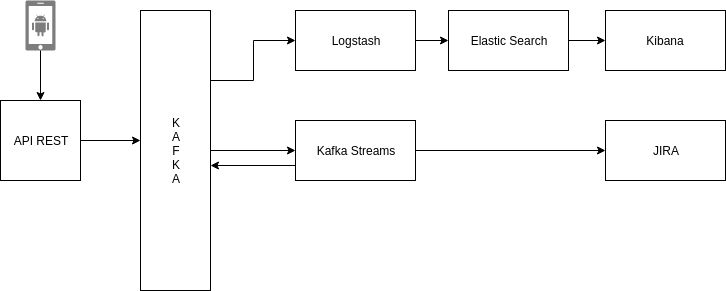
\includegraphics[width=\linewidth]{Arquitectura.png}
	\caption{Arquitectura resultante}
	\label{fig:arquitectura}
\end{figure}
%%\chapter{Integración de conocimientos}
Los conocimientos que más he integrado en este proyecto son los adquiridos en Redes de Computadores (XC), Internet Móvil (IM), Protocolos de Internet (PI), Seguridad Informática (SI), Proyectos de Tecnologías de la Información (PTI) y Administración de Sistemas Operativos (ASO).

PTI me ha ayudado a planificar la parte técnica del proyecto y a tener en cuenta aspectos como la documentación, el uso de sistemas de versiones, el plantear unos objetivos y elaborar una táctica para llevarlos a cabo.

ASO me ha ayudado a administrar las máquinas a la hora de hacer el despliegue, tener en cuenta las versiones de los programas utilizados y a elaborar scripts que automaticen ciertas partes del despliegue.

IM me ha ayudado a comprender la teoría a bajo nivel sobre la transmisión de información que hacen los dispositivos móviles, me ha hecho tener en cuenta ciertos aspectos a la hora de hacer el envío de eventos y me ha inspirado para la recolección de los eventos.

XC y PI me han ayudado a comprender todo el tema de networking del trabajo, XC sobretodo ha ayudado en la parte de definir las subredes del sistema y PI en decidir cual era la mejor opción para el módulo de recepción de eventos, a parte de ayudarme a tener en cuenta temas de redundancia y balanceo de carga.

SI me ha ayudado a tener en cuenta ciertos aspectos sobre la seguridad del proyecto así como inspirarme en la creación del sistema puesto que en la asignatura se estudian sistema que producen alertas.
 %%DONE
%%\chapter{Identificación de leyes y regulaciones}

Las dos normativas a las cuales este proyecto podría ser sensible de recibir la aplicación es la Ley Orgánica de Protección de Datos de Carácter Personal (LOPD) a nivel estatal y el Reglamento General de Protección de Datos (GDPR) a nivel europeo, pero no a tal proyecto no se le aplican dichas normativas puesto que no se están recogiendo los datos que tales leyes consideran como sensibles.

La LOPD considera datos de carácter personal: cualquier información numérica, alfabética, gráfica, fotográfica, acústica o de cualquier otro tipo concerniente a personas físicas identificadas o identificables.
En ningún caso se está recogiendo información que puede hacer al usuario identificable.

El GDPR considera datos personales todos aquellos que puedan revelar la identidad del usuario. También incluye direcciones IP pero en el presente proyecto no se recogen direcciones IP de los usuarios. %%DONE


\appendix
%% Cap'itulos incluidos despues del comando \appendix aparecen como ap'endices
%% de la tesis.
\chapter{Diagrama de Gantt} \label{cap:ganttanex}

\begin{landscape}
	\begin{figure}
		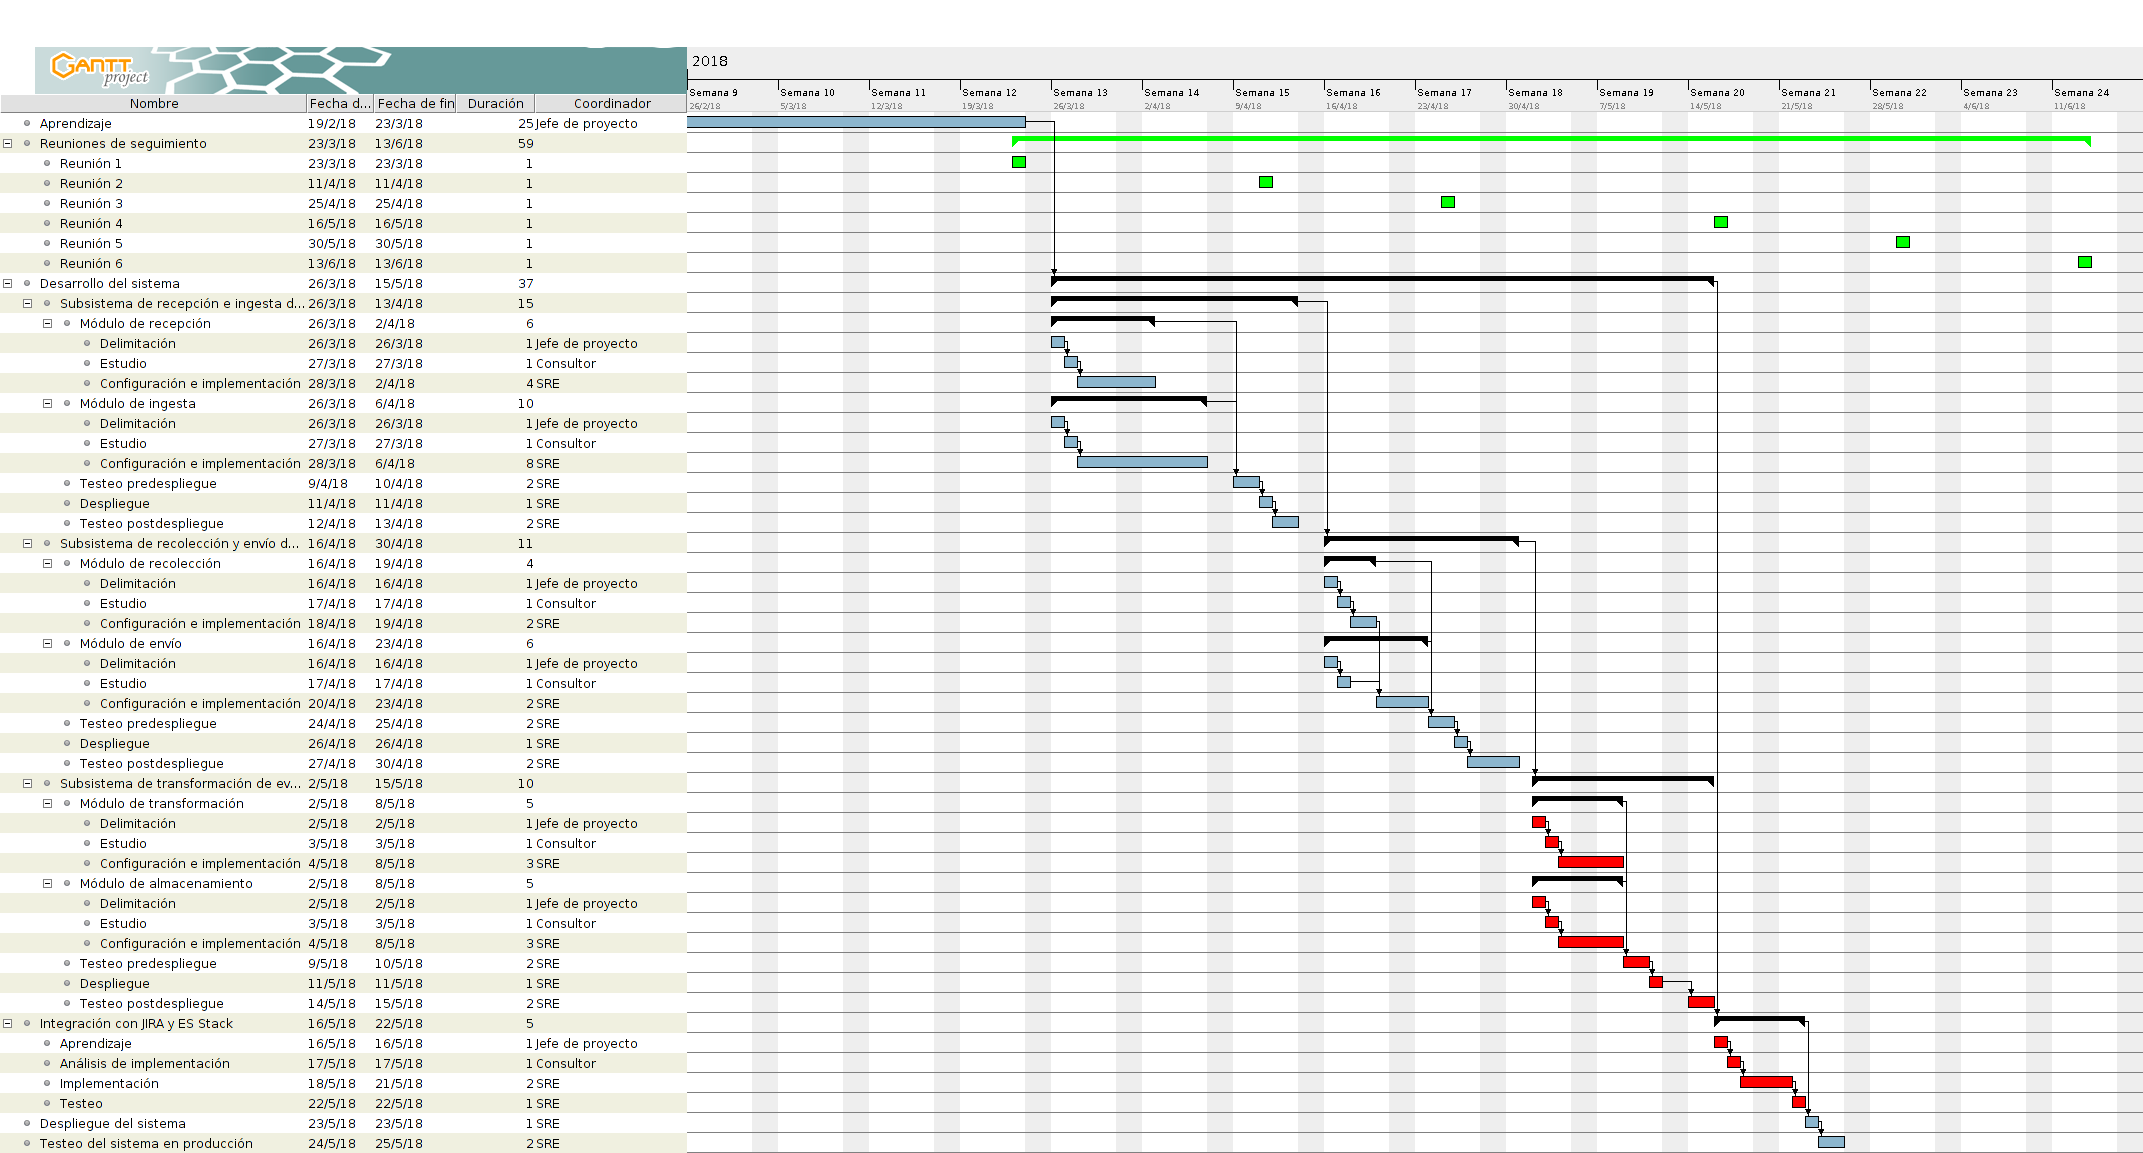
\includegraphics[width=\linewidth]{Gantt.png}
		\caption{Diagrama de Gantt Final}
		\label{fig:gantt}
	\end{figure}
\end{landscape}

\begin{landscape}
	\begin{figure}
		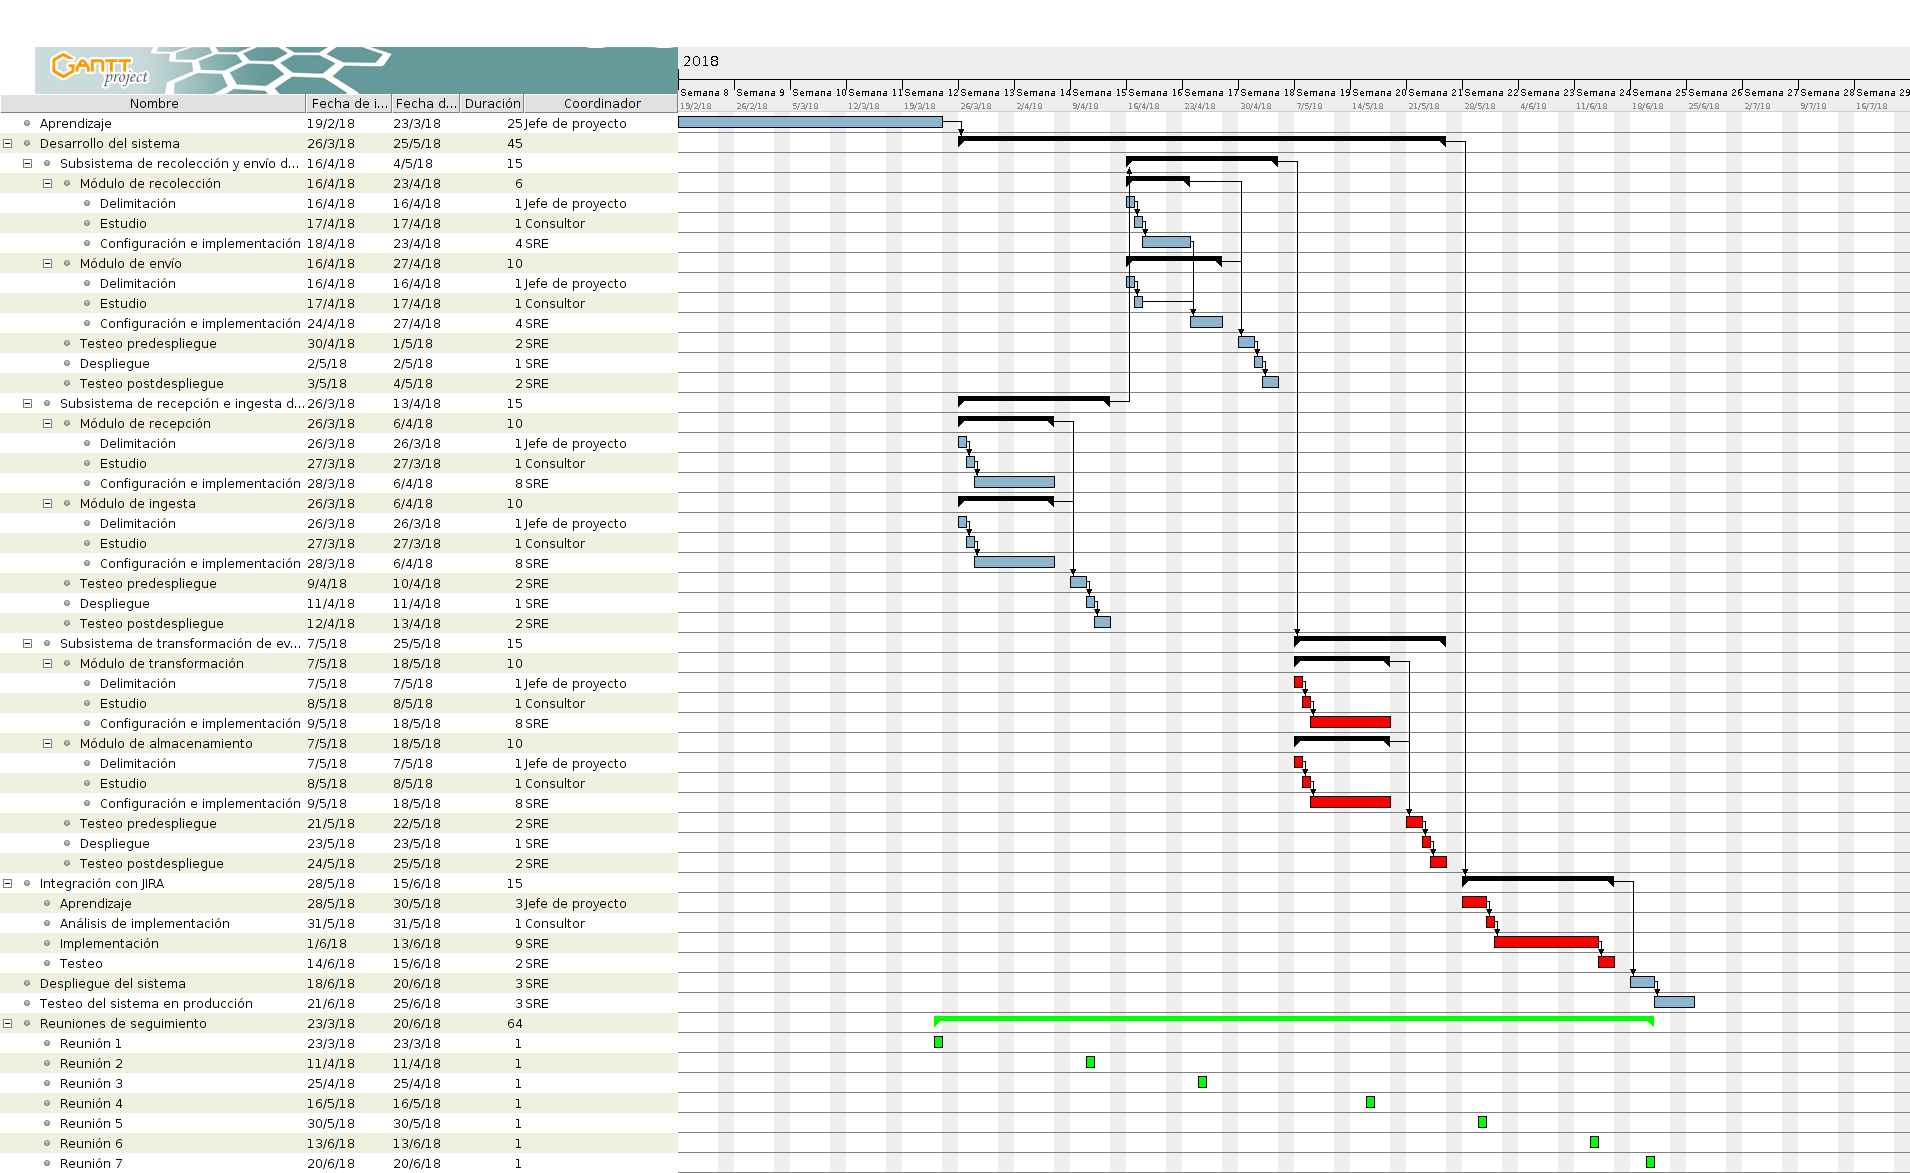
\includegraphics[width=\linewidth]{Gantt_ini.png}
		\caption{Diagrama de Gantt Inicial}
		\label{fig:ganttini}
	\end{figure}
\end{landscape}


\chapter{Leyenda diagrama de despliegue}
\begin{figure}
	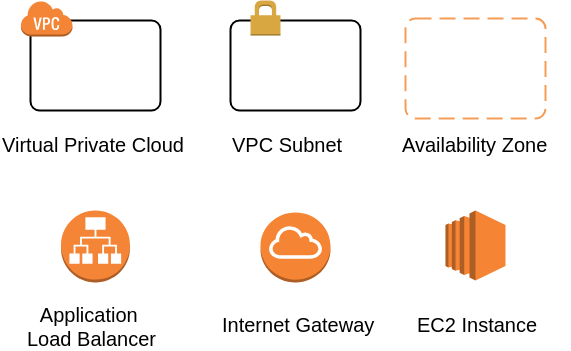
\includegraphics[width=\linewidth]{Moduloss-leyenda.png}
	\caption{Leyenda del diagrama de despliegue}
	\label{fig:leyenda}
\end{figure}
\chapter{Reproducción del sistema}

En el siguiente anexo se detalla como reproducir los módulos de recepción, ingesta, transformación y almacenamiento en un solo nodo. Algunas configuraciones difieren de las del sistema en producción por el hecho de reproducirse en solo un nodo. Se supone un nodo con Ubuntu 16.04 Server Edition y con JRE 1.8.0 instalado.

Los módulos de recepción e ingesta están compuestos por librerías de Android, el siguiente enlace es un repositorio de una aplicación Android que se ha utilizado para testear que los módulos se integran correctamente:

\href{https://github.com/pezmosca/LogBackToKafka.git}{https://github.com/pezmosca/LogBackToKafka.git}

\section{Módulo de recepción}
\subsection{Adquisición de la herramientas}
Para adquirir la herramienta de este módulo se ha de rellenar un formulario en la siguiente web:

\href{https://www.confluent.io/download/}{https://www.confluent.io/download}

Se descargará en el home de Ubuntu para simplificar la reproducción.

\subsection{Instalación de las herramientas}
La herramienta será instalada en el home de Ubuntu para simplificar la reproducción. Suponiendo que la herramienta está en el home y suponiendo la versión 4.1.1:

\begin{lstlisting}[language=Bash]
tar xzf confluent-oss-4.1.1-2.11.tar.gz
mv confluent-oss-4.1.1-2.11.tar.gz confluent

sudo systemctl enable kafka-rest.service
sudo systemctl start kafka-rest.service
\end{lstlisting}

\subsubsection{kafka-rest.service}
\begin{lstlisting}[language=Bash]
[Unit]
Description=Apache Kafka HTTP Proxy
Documentation=https://docs.confluent.io/current/kafka-rest/docs/index.html
Requires=network.target remote-fs.target
After=network.target remote-fs.target

[Service]
Type=simple
User=user
Group=user
ExecStart=/home/user/confluent/bin/kafka-rest-start /home/user/confluent/etc/kafka-rest/kafka-rest.properties
ExecStop=/home/user/confluent/bin/kafka-rest-stop

[Install]
WantedBy=multi-user.target
\end{lstlisting}

\subsection{Configuración de las herramientas}
La configuración por defecto es valida para este ejemplo.

%%%%%%%%%%%%%%%%%%%%%%%%

\section{Módulo de ingesta}
\subsection{Adquisición de las herramientas}
Se descargará en el home de Ubuntu para simplificar la reproducción.
\begin{lstlisting}[language=Bash]
wget http://apache.rediris.es/kafka/1.1.0/kafka_2.11-1.1.0.tgz
\end{lstlisting}

\subsection{Instalación de las herramientas}
La herramienta será instalada en el home para simplificar la reproducción. Suponiendo que la herramienta está en el home y suponiendo la versión 1.1.0:
\begin{lstlisting}[language=Bash]
tar xzf kafka_2.11-1.1.0.tgz
mv kafka_2.11-1.1.0.tgz kafka

sudo systemctl enable zookeeper.service
sudo systemctl start zookeeper.service

sudo systemctl enable kafka.service
sudo systemctl start kafka.service
\end{lstlisting}

\subsubsection{zookeeper.service}
\begin{lstlisting}[language=Bash]
[Unit]
Description=Apache Zookeeper server (Kafka)
Documentation=http://zookeeper.apache.org
Requires=network.target remote-fs.target 
After=network.target remote-fs.target

[Service]
Type=simple
User=user
Group=user
ExecStart=/home/user/kafka/bin/zookeeper-server-start.sh /home/user/kafka/config/zookeeper.properties
ExecStop=/home/user/kafka/bin/zookeeper-server-stop.sh

[Install]
WantedBy=multi-user.target
\end{lstlisting}

\subsubsection{kafka.service}
\begin{lstlisting}[language=Bash]
[Unit]
Description=Apache Kafka server (broker)
Documentation=http://kafka.apache.org/documentation.html
Requires=network.target remote-fs.target
After=network.target remote-fs.target

[Service]
Type=simple
User=user
Group=user
ExecStart=/home/user/kafka/bin/kafka-server-start.sh /home/user/kafka/config/server.properties
ExecStop=/home/user/kafka/bin/kafka-server-stop.sh

[Install]
WantedBy=multi-user.target
\end{lstlisting}

\subsection{Configuración de las herramientas}
La configuración por defecto es valida para este ejemplo.

%%%%%%%%%%%%%%%%%%%%%%%%

\section{Módulo de procesado}
\subsection{Adquisición de las herramientas}
Se descargará en el home de Ubuntu para simplificar la reproducción. De Kafka Streams se descargarán los jars utilizados para testear la solución, hay diversos jars para poder testear por separado cada una de las acciones que hace la aplicación con Kafka Streams, pero se podría implementar con threads en un solo jar.
\begin{lstlisting}[language=Bash]
wget https://github.com/pezmosca/empty/raw/master/jars.tar.gz
wget https://artifacts.elastic.co/downloads/logstash/logstash-6.3.0.tar.gz
\end{lstlisting}

\subsection{Instalación de las herramientas}
La herramienta será instalada en el home para simplificar la reproducción. Suponiendo que la herramienta está en el home y suponiendo la versión 6.3.0:
\begin{lstlisting}[language=Bash]
tar xzf logstash-6.3.0.tar.gz
mv logstash-6.3.0.tar.gz logstash
tar xzf jars.tar.gz

sudo systemctl enable logstash.service
sudo systemctl start logstash.service

sudo systemctl enable kafkastreams.service
sudo systemctl start kafkastreams.service
\end{lstlisting}
\subsubsection{logstash.service}
\begin{lstlisting}[language=Bash]
[Unit]
Documentation=https://www.elastic.co/products/logstash
After=network.target
ConditionPathExists=/home/ec2-user/logstash/tfg-pipeline.conf

[Service]
User=user
ExecStart=/home/user/logstash/bin/logstash -f /home/user/logstash/tfg-pipeline.conf --config.reload.automatic

[Install]
WantedBy=multi-user.target
\end{lstlisting}

\subsubsection{kafkastreams.service}
\begin{lstlisting}[language=Bash]
[Unit]
Description=Kafka Streams Service
Requires=network.target remote-fs.target
After=network.target remote-fs.target

[Service]
User=user
Group=user
ExecStart=/home/user/jars/start.sh

[Install]
WantedBy=multi-user.target
\end{lstlisting}

\subsection{Configuración de las herramientas}
La configuración por defecto no es valida para este ejemplo, se ha de generar una pipeline para Logstash.


\subsubsection{Logstash}
Se ha de generar una pipeline para procesar los eventos. Tal pipeline se ha de crear en ~/logstash/tfg-pipeline.conf y el contenido ha de ser el siguiente:

\begin{lstlisting}
input {
  kafka {
    bootstrap_servers => "localhost:9092"
    topics => ["log", "crashout"]
    group_id => "tfg-logstash"
    codec => json
    decorate_events => true
  }
}

filter {
  if [@metadata][kafka][topic] == "log" {
    mutate {
      rename => { "T" => "ExecutionTime"
      "T2" => "Timestamp"
      "L" => "Level"
      "TN" => "ThreadName"
      "LN" => "Class"
      "M" => "Message"
      }
    }
  }
}

output {

  if[@metadata][kafka][topic] == "log" {
    elasticsearch {
      hosts => [ "localhost:9200" ]
      index => "logs"
    }
  }


  if[@metadata][kafka][topic] == "crashout" {
    elasticsearch {
      hosts => [ "localhost:9200" ]
      index => "crashes"
    }
  }
}
\end{lstlisting}

%%%%%%%%%%%%%%%%%%%%%%%%

\section{Módulo de almacenamiento}
\subsection{Adquisición de las herramientas}
Las herramientas para este módulo se descargarán en el home de Ubuntu para simplificar la reproducción.
\begin{lstlisting}[language=Bash]
wget https://artifacts.elastic.co/downloads/elasticsearch/elasticsearch-6.3.0.tar.gz
wget https://artifacts.elastic.co/downloads/kibana/kibana-6.3.0-linux-x86_64.tar.gz
\end{lstlisting}

\subsection{Instalación de las herramientas}
Las herramientas serán instalada en el home para simplificar la reproducción, suponiendo que las herramientas están en el home y suponiendo la versión 6.3.0 de Elastic Search, Logstash y Kibana, y la 7.10.1 de JIRA. Para adquirir JIRA se ha de acceder mediante un navegador web a \href{https://es.atlassian.com/software/jira/download}{https://es.atlassian.com/software/jira/download} y descargarlo.
\begin{lstlisting}[language=Bash]
tar xzf elasticsearch-6.3.0.tar.gz
mv elasticsearch-6.3.0.tar.gz elasticsearch

tar xzf kibana-6.3.0.tar.gz
mv kibana-6.3.0.tar.gz kibana

sudo systemctl enable elasticsearch.service
sudo systemctl enable kibana.service

sudo chmod +x atlassian-jira-software-7.10.1-x64.bin
sudo ./atlassian-jira-software-7.10.1-x64.bin
\end{lstlisting}

\subsubsection{elasticsearch.service}\label{cap:elasticsearch}
\begin{lstlisting}[language=Bash]
[Unit]
Documentation=https://www.elastic.co/products/elasticsearch
After=network.target

[Service]
User=user
Group=user
LimitMEMLOCK=infinity
LimitNOFILE=65536
ExecStart=/home/user/elasticsearch/bin/elasticsearch

[Install]
WantedBy=multi-user.target
\end{lstlisting}

\subsubsection{kibana.service}\label{cap:kibana}
\begin{lstlisting}[language=Bash]
[Unit]
Description=Kibana
After=network.target

[Service]
ExecStart=/home/user/kibana/bin/kibana
Type=simple
Restart=always

[Install]
WantedBy=default.target
\end{lstlisting}


\subsection{Configuración de las herramientas}
La configuración por defecto es valida para este ejemplo.







%%\chapter{Encuesta conocimientos y competencias en sostenibilidad}
Una vez contestada la encuesta me he dado cuenta de que no he tenido en mente muchos aspectos de sostenibilidad bastante importantes. Por un lado desconocía toda la literatura detrás de la sostenibilidad y los modelos existentes, desconocía el hecho de poder medir cómo de sostenible se es. Mi desconocimiento de la materia en parte puede deberse a que ya llevo años trabajando en la industria y en las empresas que he estado no se ha hecho mucho hincapié en los aspectos de sostenibilidad. Después de haber hecho la encuesta considero que ya empiezo a entender mejor los aspectos que engloba la sostenibilidad y ya empiezo a tenerlos en cuenta en el proyecto, muchos de los aspectos son de sentido común, cosa que puede hacer que se piense que ya se tienen en cuenta cuando se propone un proyecto, pero hay otros aspectos más profundos que es interesante estudiarlos. Por lo que en resumen, mi conocimiento del tema era bastante limitado y me he dado cuenta de que debo de tener en cuenta factores en mi proyecto que pueden ayudar a que este sea sostenible.
Con respecto la calidad de la encuesta, aunque cumple una función de concienciación importante, es mejorable a nivel organizativo. Quizás permitir respuestas más abiertas a las preguntas y organizar las preguntas en subsecciones puede facilitar el hacer resúmenes autoevaluativos posteriormente y darte cuenta qué puntos fuertes y débiles tienes con respecto al tema de la sostenibilidad.
Concluyendo, he de documentarme mejor sobre el tema de la sostenibilidad, no solo porque sea obligación de GEP sino porque es algo importante a nivel social dado que el proyecto tiene un impacto en la sociedad y me he de esforzar de que sea un impacto positivo.
%\include{apendiceB}
%\include{apendiceC}

%% Incluir la bibliograf'ia. Mirar el archivo "biblio.bib" para m'as detales
%% y un ejemplo.
\bibliographystyle{unsrt}
\bibliography{biblio}

\end{document}
